% !TeX encoding = UTF-8
% !TeX program = xelatex
% !TeX spellcheck = en_US

\documentclass[twoside]{article}

\usepackage{geometry}
\geometry{
    paperwidth = 155mm,
    paperheight = 235mm,
    outer = 20mm,
    inner = 20mm,
    top = 25mm,
    bottom = 20mm
}

% fonts & unicode
\usepackage[PunctStyle=kaiming]{xeCJK}
\usepackage{amsmath}
\usepackage{unicode-math}

\setCJKmainfont{NotoSerifCJKsc-Regular.otf}[
    Path            = ../../fonts/,
    BoldFont        = NotoSansCJKsc-Medium.otf,
    ItalicFont      = fzktk.ttf,
    Scale           = .97,
    ItalicFeatures  = {Scale = 1}
]

\setCJKsansfont{NotoSansCJKsc-DemiLight.otf}[
    Path            = ../../fonts/,
    BoldFont        = NotoSansCJKsc-Bold.otf,
    Scale           = .97
]

\setCJKmonofont{NotoSansCJKsc-DemiLight.otf}[
    Path            = ../../fonts/,
    BoldFont        = NotoSansCJKsc-Bold.otf,
    Scale           = .9
]

\newCJKfontfamily{\KaiTi}{fzktk.ttf}[
    Path            = ../../fonts/,
    BoldFont        = NotoSansCJKsc-Medium.otf,
    BoldFeatures    = {Scale = .97},
    ItalicFont      = NotoSerifCJKsc-Regular.otf,
    ItalicFeatures  = {Scale = .97}
]

\setmainfont{XITS}[
    Path            = ../../fonts/,
    Extension       = .otf,
    UprightFont     = *-Regular,
    BoldFont        = *-Bold,
    ItalicFont      = *-Italic,
    BoldItalicFont  = *-BoldItalic
]

\setsansfont{Lato}[
    Path            = ../../fonts/,
    Scale           = MatchUppercase,
    Extension       = .ttf,
    UprightFont     = *-Regular,
    BoldFont        = *-Bold,
    ItalicFont      = *-Italic,
    BoldItalicFont  = *-BoldItalic
]

\setmonofont{FiraMono}[
    Path            = ../../fonts/,
    Scale           = .9,
    Extension       = .otf,
    UprightFont     = *-Regular,
    BoldFont        = *-Bold
]

\setmathfont{XITSMath-Regular.otf}[
    Path            = ../../fonts/,
    BoldFont        = XITSMath-Bold.otf
]

\setmathfont{latinmodern-math.otf}[
    Path            = ../../fonts/,
    range           = {frak, bffrak},
    BoldFont        = latinmodern-math.otf
]

\setmathfont{LatoMath.otf}[
    Path            = ../../fonts/,
    Scale           = .95,
    BoldFont        = LatoMath.otf,
    version         = sf
]

\setmathfont{LatoMath.otf}[
    Path            = ../../fonts/,
    Scale           = .95,
    BoldFont        = LatoMath.otf,
    range           = {bb, sfup -> up, sfit -> it, bfsfup -> bfup, bfsfit -> bfit}
]

\setmathfont{STIX2Math.otf}[
    Path            = ../../fonts/,
    BoldFont        = STIX2Math-Bold.otf,
    range           = {\int, \sum, \prod, \coprod, \bigoplus, \bigotimes, \bigcup, \bigcap, \bigvee, \bigwedge}
]

\Umathcode`/  =  "0 "0 "2215    % / -> U+2215 division slash

% spacing
\AtBeginDocument{
    \hfuzz=2pt
    \emergencystretch 2em
    \setlength{\belowdisplayshortskip}{\belowdisplayskip}
}

% parts
\usepackage{tikz}

\renewcommand{\titlepage}[2]{%
    \clearpage%
    \thispagestyle{empty}%
    \vspace*{20mm}%
    \centerline{\begin{tikzpicture}
        \node [scale = 3] at (0, 0) {\sffamily 荷\hspace{.5em}思};
        \node [scale = 1.8] at (0, -94.5mm) {\sffamily #1};
        \node [scale = 1.2] at (0, -105mm) {\sffamily #2};
        \draw (-16mm, -8mm) -- (16mm, -8mm);
        \draw (-14mm, -100mm) -- (14mm, -100mm);
        \draw (-13mm, -110mm) -- (13mm, -110mm);
    \end{tikzpicture}}%
    \clearpage%
}

\newcommand{\committee}{%
    \clearpage%
    \thispagestyle{empty}%
    \vspace*{120mm}%
}

\newcommand{\committeeitem}[2]{%
    \par%
    {%
        \leftskip=3em%
        \rightskip=8em%
        \parindent=-3em%
        {\bfseries\sffamily#1}\quad%
        {\sffamily#2}%
        \par\vspace{6pt}%
    }%
}

\newcommand{\toctitle}{%
    \clearpage%
    \thispagestyle{empty}%
    \vspace*{15mm}%
    \noindent{\huge\sffamily 目录}%
    \par\vspace{10mm}%
}

\newcommand{\tocsection}[1]{%
    \par\vspace{6mm}%
    \noindent{\large\sffamily #1}%
    \par\vspace{4mm}%
}

\newcommand{\tocitem}[3]{%
    \par%
    {%
        \leftskip=3em%
        \parindent=-3em%
        \makebox[2em][r]{\textbf{\textsf{#3}}}%
        \quad#1%
        \hfill\mbox{}\hfill\phantom{#2}\hfill\makebox[0em][r]{#2}%
        \par\vspace{8pt}%
    }%
}

% Make total pages even
\usepackage[strict]{changepage}

\AtEndDocument{%
  \checkoddpage\ifoddpage\newpage\thispagestyle{empty}\mbox{}\fi
}

\def\term#1{\textbf{#1}}

\theoremstyle{definition}
\newtheorem*{convention}{Convention}

\makeatletter
\newcommand\dif{%  % 微分符号
  \mathop{}\!%
  \ifthu@math@style@TeX
    d%
  \else
    \mathrm{d}%
  \fi
}

\def\f{\mathbf{f}}
\def\Z{\mathbb{Z}}
\def\Q{\mathbb{Q}}
\def\ttb{\mathtt{b}}
\def\abs#1{\left|#1\right|}
\def\K{\mathbb{k}}
\def\NH{\mathit{NH}}
\def\bi{\mathbf{1}}
\def\ii{\boldsymbol{i}}
\def\:{\colon}
\def\rad{\operatorname{rad}}
\def\soc{\operatorname{soc}}
\def\Hom{\operatorname{Hom}}
\def\ext{\operatorname{ext}}
\def\Ext{\operatorname{Ext}}
\def\Dim{\operatorname{Dim}}
\def\KP{\operatorname{KP}}
\def\mod{\mathsf{mod}}
\def\fmod{\mathsf{fmod}}
\def\pmod{\mathsf{pmod}}
\def\Ch{\operatorname{Ch}}
\def\*{\circledast}
\def\ox{\otimes}
\def\ex{\boxtimes}
\def\Ind{\operatorname{Ind}}
\def\Res{\operatorname{Res}}
\def\9{\left(}
\def\0{\right)}
\def\<{\left<}
\def\>{\right>}
\def\std{\increment}
\def\pstd{\overline{\std}}
\def\pcostd{\overline{\nabla}}
\def\costd{\nabla}
\def\im{\operatorname{im}}
\def\End{\operatorname{End}}
\def\Aut{\operatorname{Aut}}
\def\LL{\mathscr{L}}
\def\D{\mathscr{D}}
\def\OO{\mathscr{O}}
\def\pt{\mathrm{pt}}
\def\IC{\mathrm{IC}}

\usepackage[shortlabels]{enumitem}

\addbibresource{ref.bib}

\begin{document}

\title{Cluster Category as Perfect Derived Category}
\author{Fan Li\footnote{范俐,清华大学数学科学系数71班.}}
\begin{abstract}
  Calabi--Yau algebras and categories play important roles in cluster theory
  and quiver representation theory.
  We first review some basic notions on
  quiver representations and cluster categories via orbit categories.
  We then generalize some notions and conclusions about Calabi--Yau completion
  in the sense of Keller.
  We also discuss the generalized cluster theory via Verdier quotient.
  Finally, for a finite-dimensional dg $\Bk$-algebra $A$ of finite global dimension,
  we give a triangle equivalence $\per A \cong \Ce(\Pi_{\mathbb{X}}A)$ between
  $\mathbb{X}$-cluster category and perfect derived category of $A$.

  \bigskip
  \noindent
  \textbf{Keywords:}
  perfect derived categories; cluster category; Calabi-Yau category
\end{abstract}

\tableofcontents

\section{Introduction}
% \subsection{Conformal field theory}

% A \emph{conformal field theory} in two dimensions
% is a two dimensional quantum field theory that is
% invariant under conformal transformations.

% Consider a conformal field theory on
% the space-time cylinder $S^1 \times \bbR$,
% where $S^1$ is the space component and $\bbR$ is the time component.
% We use the complex coordinate $\xi = \theta + \upi \tau$,
% where $\theta \in S^1$ and $\tau \in \bbR$.
% We then change the coordinates to
% \[
%     z = \upe^{-\upi \xi}.
% \]
% This maps the cylinder to the set $\bbC \setminus \{ 0 \}$,
% and the time ordering becomes the radial ordering
% of concentric circles centred at the origin.

% \figplacehold


\subsection{Definition}

First of all,
we briefly recall the definition of a vertex algebra.
For details, we refer the reader to
\cite{frenkel-ben-zvi} and \cite{kac}.

\begin{definition}
    A \emph{vertex algebra} is the data $(\scrV, Y, T, \ket{0})$, where
    \begin{itemize}
        \item
            $\scrV$ is a $\bbZ_2$-graded vector space over $\bbC$,
            called the \emph{state space},
            or the \emph{space of observables}.
        \item
            $\ket{0} \in \scrV$ is an even element,
            called the \emph{vacuum state}.
        \item
            $Y$ is an even linear map
            \begin{align*}
                Y \colon \scrV & \to \End(\scrV) [[z, z^{-1}]], \\
                A & \mapsto A (z) = \sum_{n \in \bbZ} A_{(n)} z^{-n - 1},
            \end{align*}
            called the \emph{state--field correspondence}.
        \item
            $T \colon \scrV \to \scrV$
            is an even endomorphism,
            called the \emph{translation operator}.
    \end{itemize}
    They satisfy the following axioms:
    \begin{itemize}
        \item
            For all $A, B \in \scrV$, we have
            \[
                A (z) \, B \in \scrV ((z)),
            \]
            where $\scrV ((z)) = \scrV [[z]] [z^{-1}]$
            is the space of formal Laurent series
            with values in $\scrV$.
            In other words, we have
            \[
                A_{(n)} B = 0 \quad (n \gg 0).
            \]
            
        \item
            (Vacuum)
            $T \ket{0} = 0$
            and $\ket{0} (z) = \operatorname{id}$.
            For all $A \in \scrV$,
            $A (z) \ket{0} = A + O (z)$.
            
        \item
            (Translation)
            For all $A \in \scrV$, we have $[T, A(z)] = \partial_z A(z)$.
            
        \item
            (Locality)
            For all $A, B \in \scrV$, there exists $N \in \bbN$ such that
            \[
                (z - w)^N [A(z), B(w)] = 0.
            \]
    \end{itemize}
    By abuse of language,
    we say that $\scrV$ is a vertex algebra.
    \varqed
\end{definition}

For $A \in \scrV$, note that the operator $A_{(n)} \in \End (\scrV)$
can be expressed as a residue:
\[
    A_{(n)} = \operatorname{Res}_{z = 0} (z^n A(z)).
\]

\begin{definition}
    A \emph{graded vertex algebra}
    is a vertex algebra $\scrV$,
    together with a $\bbZ$-grading
    \[
        \scrV = \bigoplus_{m} \scrV_m
    \]
    on the vector space $\scrV$, compatible with the $\bbZ_2$-grading
    (i.e.\ the two gradings form a $\bbZ \times \bbZ_2$-bigrading),
    such that
    \begin{itemize}
        \item
            $\ket{0} \in \scrV_0$.
        \item
            $\deg T = 1$.
        \item
            For any $A \in \scrV_m$,
            we have $\deg A_{(n)} = -n - 1 + m$.
    \end{itemize}
    If $A \in \scrV_m$,
    we say that $A$ has \emph{conformal dimension} $m$.
    \varqed
\end{definition}

\begin{definition}
    A \emph{conformal vertex algebra},
    also called a \emph{vertex operator algebra},
    is a graded vertex algebra $\scrV$,
    together with an even element $L \in \scrV_2$,
    called the \emph{conformal vector},
    such that if we write
    \[
        L (z) = \sum _{n \in \bbZ} L_{n} z^{-n-2}
    \]
    (that is, $L_n = L_{(n+1)}$, so that $\deg L_n = -n$), then
    \begin{itemize}
        \item
            $L_{-1} = T$ is the translation operator.
        \item
            For all $m$, $\scrV_m$ is the $m$-eigenspace of $L_0$.
        \item
            We have the \emph{Virasoro relations}
            \[
                [L_n, L_m] =
                (n - m) L_{n + m} +
                c \cdot \frac{n^3 - n}{12} \cdot \delta_{n, -m},
            \]
            where $c \in \bbC$ is called the \emph{central charge}.
            \varqed
    \end{itemize}
\end{definition}


\subsection{Operator product expansion}

The analogue between associative algebras and vertex algebras
can be formulated as follows.
For an associative algebra $V$, each element $A \in V$
defines an element of $\End (V)$ by left multiplication,
so the structure of the algebra is given by a linear map
\begin{align*}
    Y \colon V & \to \End (V), \\
    A & \mapsto A \cdot {-}.
\end{align*}
In a vertex algebra $\scrV$, there is a family of multiplication operators,
parametrized by the formal variable $z$,
and the structure of the vertex algebra is given by
\begin{align*}
    Y \colon \scrV & \to \End(\scrV) [[z, z^{-1}]], \\
    A & \mapsto A (z) \cdot -.
\end{align*}

From this point of view,
one can talk about whether a vertex algebra
is associative.
It turns out that all vertex algebras
are associative in the following sense.

\begin{theorem}
    \label{thm-assoc}
    Let $\scrV$ be a vertex algebra,
    and let $A, B, C \in \scrV$. 
    \begin{itemize}
        \item
            \textup{(Associativity)}
            The elements
            \begin{align*}
                A (z) \, B (w) \, C
                & \in \scrV ((z)) ((w)), \\
                B (w) \, A (z) \, C
                & \in \scrV ((w)) ((z)), \\
                (A (z - w) \, B) (w) \, C
                & \in \scrV ((w)) ((z - w))
            \end{align*}
            come from the same element of
            \[
                \scrV [[z, w]] [z^{-1}, w^{-1}, (z-w)^{-1}],
            \]
            where the inclusions
            \begin{align*}
                \scrV [[z, w]] [z^{-1}, w^{-1}, (z-w)^{-1}]
                & \hookrightarrow \scrV ((z)) ((w)), \\
                \scrV [[z, w]] [z^{-1}, w^{-1}, (z-w)^{-1}]
                & \hookrightarrow \scrV ((w)) ((z)), \\
                \scrV [[z, w]] [z^{-1}, w^{-1}, (z-w)^{-1}]
                & \hookrightarrow \scrV ((w)) ((z-w))
            \end{align*}
            are given by
            \begin{align*}
                (z-w)^{-1} & \mapsto
                \frac{1}{z} \sum_{n=0}^\infty
                \biggl( \frac{w}{z} \biggr)^n, \\
                (z-w)^{-1} & \mapsto
                -\frac{1}{w} \sum_{n=0}^\infty
                \biggl( \frac{z}{w} \biggr)^n, \\
                z^{-1} & \mapsto
                \frac{1}{w} \sum_{n=0}^\infty
                \biggl( \frac{w-z}{w} \biggr)^n,
            \end{align*}
            respectively.
    \end{itemize}
\end{theorem}

See \cite[Theorem~3.2.1]{frenkel-ben-zvi}.

As a result,
we may write down equations of the form
\[
    A (z) \, B (w) =
    \sum_{n \in \bbZ} \frac{(A_{(n)} B) (w)}{(z - w)^{n+1}},
\]
or sometimes, we only write down the singular part:
\[
    A (z) \, B (w) =
    \sum_{n = 0}^N \frac{(A_{(n)} B) (w)}{(z - w)^{n+1}}
    + \text{reg.},
\]
where `reg.'\ means `regular part'.
These formulas are known as the
\emph{operator product expansion}, or the \emph{OPE},
of the fields $A$ and $B$
\cite[\S3.3]{frenkel-ben-zvi}.

Note that technically,
the OPE formulas only make sense in the space
\[
    \scrV [[z, w]] [z^{-1}, w^{-1}, (z-w)^{-1}].
\]

From the OPE, we can recover the commutation relations
of vertex operators.
Indeed, for even elements $A, B \in \scrV$, we have
\begin{align*}
    \oint_w A (z) \, B (w) \, d z
    & = \oint_{\gamma_1} A (z) \, B (w) \, d z
    - \oint_{\gamma_2} B (w) \, A (z) \, d z \\
    & = \Biggl[ \ \oint A \ , B (w) \Biggr],
\end{align*}
where $\oint_w$ denotes the contour integral
along a small circle around $w$;
$\gamma_1, \gamma_2$ are as shown in the following picture;
and $\oint A$ is short for $\oint_0 A (z) \, d z$,
and is equal to $2 \uppi \upi \, A_{(0)}$.

\[
    \begin{tikzpicture}[
        thick,
        decoration = {
            markings,
            mark = at position 0.05 with {\arrow[scale=1.5]{stealth}}
        },
        scale = .8
    ]
        \begin{scope}
            \fill (0, 0) circle (.07);
            \fill (1.8, 1.8) circle (.07);
            \draw[postaction = {decorate}] (1.8, 1.8) circle (.6);
            \draw[postaction = {decorate}] (0, 0) circle (3.6);
            \draw[postaction = {decorate}] (0, 0) circle (1.4);
            \node at (.25, -.15) {$0$};
            \node at (2.05, 1.65) {$w$};
            \node at (1.7, .1) {$\gamma_2$};
            \node at (3.8, .8) {$\gamma_1$};
        \end{scope}
    \end{tikzpicture}
\]

Integrating over $w$, we obtain the formula
for the commutator of $\oint A$ and $\oint B$:
\[
    \Biggl[ \ \oint A \ , \ \oint B \Biggr] =
    \oint_0 \ d w \ 
    \oint_w \ d z \ A (z) \, B (w).
\]
See also \cite[Ch.~6]{cft}.
A similar argument shows that this holds for odd elements as well.

We can slightly generalize this argument,
by replacing the integrand $A (z) \, B (w)$
by $z^m w^k \, A (z) \, B (w)$.
Then one arrives at the following result,
a version of which was taken as
one of the axioms in Borcherd's original definition
\cite{borcherds86} of a vertex algebra.

\begin{theorem} [Borcherd's identity]
    For any $A, B \in \scrV$ and $m, k \in \bbZ$, we have
    \[
        [A_{(m)}, B_{(k)}] =
        \sum_{n \geq 0} \binom{m}{n} \,
        (A_{(n)} B)_{(m+k-n)}.
    \]
    In particular, when $m = 0$, we have
    \[
        [A_{(0)}, B_{(k)}] =
        (A_{(0)} B)_{(k)}.
    \]
\end{theorem}

See also \cite[\S3.3]{frenkel-ben-zvi}
for a generalization.

\begin{proof}
    \allowdisplaybreaks
    We have
    \begin{align*}
        [A_{(m)}, B_{(k)}]
        & = \frac {1} {(2 \uppi \upi)^2}
        \Biggl[ \ 
            \oint_0 \ z^m A (z) \, d z \ , \ 
            \oint_0 \ w^k B (w) \, d w
        \Biggr] \\
        & = \frac {1} {(2 \uppi \upi)^2}
        \oint_0 \ w^k \, d w \ 
        \oint_w z^m \, d z \, A (z) \, B (w) \\
        & = \frac {1} {(2 \uppi \upi)^2}
        \oint_0 \ w^k \, d w \sum_{n \in \bbZ} \ 
        \oint_w \frac{z^m}{(z - w)^{n+1}} \, d z \,
        (A_{(n)} B) (w) \\
        & = \frac {1} {2 \uppi \upi}
        \oint_0 \ w^k \, d w \sum_{n \geq 0} \,
        \binom{m}{n} \, w^{m-n} \,
        (A_{(n)} B) (w) \\
        & = \sum_{n \geq 0} \binom{m}{n} \,
        (A_{(n)} B)_{(m+k-n)}. \qedhere
    \end{align*}
\end{proof}

Note that only the singular part of the OPE $A (z) \, B (w)$
is used in this identity.

On the other hand,
the non-singular part of the OPE
is equal to the normally ordered product,
which we now define following \cite[\S2.2]{frenkel-ben-zvi}.

\begin{definition}
    Let $\scrV$ be a vertex algebra, and let $A, B \in \scrV$.
    The \emph{normally ordered product} of the fields
    $A (z)$ and $B (w)$ is defined by the formula
    \[
        \nord{A (z) \, B (w)} =
        A (z)_+ \, B (w) + B (w) \, A (z)_-,
    \]
    where
    \[
        A (z)_+ = \sum_{n < 0} A_{(n)} z^{-n-1}, \quad
        A (z)_- = \sum_{n \geq 0} A_{(n)} z^{-n-1},
    \]
    where the plus/minus signs refer to the positive/negative powers of $z$.
    
    More generally, for $A_1, \dotsc, A_n \in \scrV$, with $n > 2$,
    the \emph{normally ordered product} of the fields
    $A_1 (z_1)$, $\dotsc$, $A_n (z_n)$ is defined inductively by
    \[
        \nord{A_1 (z_1) \cdots A_n (z_n)} =
        \nord{A_1 (z_1) \ \bigl( \nord{A_2 (z_2) \cdots A_n (z_n)} \bigr) }.
        \varqedhere
    \]
\end{definition}

The idea behind the normally ordered product is that
by changing the order of multiplication,
we avoid the singularities that we would
normally get in the OPE.
This is shown by the following theorem.

\begin{theorem}
    Let $\scrV$ be a vertex algebra, and let $A, B \in \scrV$. Then
    \[
        A (z) \, B (w) =
        \sum_{n \geq 0} \frac {(A_{(n)} B)(w)} {(z - w)^{n + 1}}
        + \nord{A (z) \, B (w)}.
    \]
    That is, the regular part of the OPE $A (z) \, B (w)$
    is exactly the normally ordered product $\nord{A (z) \, B (w)}$.
\end{theorem}

See \cite[\S3.3.6]{frenkel-ben-zvi}.

Since the normally ordered product $\nord{A (z) \, B (w)}$
is no longer singular along the diagonal $z = w$,
one may consider its restriction to the diagonal,
which is a well-defined field,
denoted by $\nord{A (z) \, B (z)}$.
This works for more than two fields as well.

Finally, we mention a theorem
that describes the field corresponding to
the product of vertex operators.
This result shows that the information of a vertex algebra
can be recovered from its generating elements.

\begin{theorem}
    \label{thm-structure}
    Let $\scrV$ be a vertex algebra, let $A^1, \dotsc, A^k \in \scrV$,
    and let $n_1, \dotsc, n_k \in \bbZ_{<0}$. Then
    \[
        \bigl( A^1_{(n_1)} \cdots A^k_{(n_k)} \ket{0} \bigr) (z) =
        \Biggl( \prod_{i=1}^k \frac{1}{(-n_i - 1)!} \Biggr) \ 
        \nord{ \partial_z^{-n_1 - 1} A^1 (z) \cdots \partial_z^{-n_k - 1} A^k (z) }.
    \]
\end{theorem}

See \cite[Corollary~4.4]{kac}.


\subsection{Examples}
\label{sect-voa-examples}

\begin{example} [$\betagamma$ system]
    \allowdisplaybreaks
    \label{eg-beta-gamma}
    Let 
    \[
        \frg^\betagamma \enspace = \enspace 
        \bigoplus_{n \in \bbZ} \bbC \cdot \beta_n
        \enspace \oplus \enspace \bigoplus_{n \in \bbZ} \bbC \cdot \gamma_n
        \enspace \oplus \enspace \bbC \cdot \mathbf{1}
    \]
    be a Lie algebra defined by
    \[
        [\beta_n, \gamma_m] = \delta_{n, -m} \cdot \mathbf{1}, \quad
        [\beta_n, \beta_m] = [\gamma_n, \gamma_m] = [\mathbf{1}, -] = 0.
    \]
    Let
    \[
        \scrV^\betagamma =
        U (\frg^\betagamma) \cdot \ket{0} \Bigg/
        \left\{ \ 
            \begin{aligned}
                \beta_n \cdot \ket{0} &= 0 \quad (n \geq 0) \\
                \gamma_n \cdot \ket{0} &= 0 \quad (n > 0) \\
                \mathbf{1} \cdot \ket{0} &= \ket{0}
            \end{aligned}
        \ \right\}
    \]
    be a representation of $\frg^\betagamma$
    generated by the vector $\ket{0}$.
    By the PBW theorem,
    as a vector space, one may identify
    \[
        \scrV^\betagamma \simeq
        \bbC [
            \beta_{-1}, \beta_{-2}, \dotsc,
            \gamma_0, \gamma_{-1}, \gamma_{-2}, \dotsc
        ].
    \]
    We assign a $\bbZ$-grading to $\scrV^\betagamma$ by
    \[
        \deg \beta_{n} = -n \ (n < 0), \quad
        \deg \gamma_{n} = -n \ (n \leq 0).
    \]
    This grading is well-defined because the elements
    $\beta_n$ ($n < 0$) and $\gamma_n$ ($n \leq 0$)
    commute with each other in $\frg^\betagamma$.
    
    We wish to define a vertex algebra structure on $\scrV^\betagamma$,
    that is, to define the maps $Y$ and $T$. Write
    \begin{align*}
        \beta (z) &= \sum_{n \in \bbZ} \beta_n z^{-n - 1}, \\
        \gamma (z) &= \sum_{n \in \bbZ} \gamma_n z^{-n}.
    \end{align*}
    In light of Theorem~\ref{thm-structure},
    we define
    \begin{align*}
        \beta_{-n-1} (z) &=
        \frac{1}{n!}
        \biggl( \frac {\partial} {\partial z} \biggr)^n \beta (z), \\
        \gamma_{-n} (z) &=
        \frac{1}{n!}
        \biggl( \frac {\partial} {\partial z} \biggr)^n \gamma (z)
    \end{align*}
    for $n \geq 0$, and for a general element
    $x_1 \cdots x_p \ket{0} \in \scrV^\betagamma$,
    where each $x_i$ is either 
    $\beta_{n}$ ($n < 0$) or $\gamma_{n}$ ($n \leq 0$),
    we define
    \[
        \bigl( x_1 \cdots x_p \ket{0} \bigr) (z) =
        \nord{ x_1 (z) \cdots x_p (z) }
    \]
    to be the normally ordered product.
    
    The commutation relations of $\beta_n$ and $\gamma_n$
    can be rewritten as the OPE
    \[
        \beta(z) \, \gamma(w) = \frac{1}{z - w} + \text{reg.}
    \]
    
    The conformal structure on $\scrV^\betagamma$ is given by the field
    \[
        L (z) = \nord{ \gamma'(z) \, \beta(z) }.
    \]
    One can show that $L$ satisfies the axioms for a conformal vertex algebra,
    and the central charge is $c = 2$. \varqed
\end{example}


\begin{example} [$\bc$ system]
    \label{eg-bc}
    The $\bc$ system is the fermionic counterpart of the $\betagamma$ system.
    Let
    \[
        \frg^\bc \enspace = \enspace 
        \bigoplus_{n \in \bbZ} \bbC \cdot b_n
        \enspace \oplus \enspace \bigoplus_{n \in \bbZ} \bbC \cdot c_n
        \enspace \oplus \enspace \bbC \cdot \mathbf{1}
    \]
    be a Lie superalgebra,
    with all the elements $b_n, c_n$ being odd, and with
    \[
        [b_n, c_m] = \delta_{n, -m} \cdot \mathbf{1}, \quad
        [b_n, b_m] = [c_n, c_m] = [\mathbf{1}, -] = 0.
    \]
    We then copy the construction of the $\betagamma$ vertex algebra
    word by word, with $b_n$ and $c_n$ in place of $\beta_n$ and $\gamma_n$,
    except that these elements are now odd.
    This defines a conformal vertex algebra
    $\scrV^\bc$, with
    \[
        b(z) \, c(w) = \frac{1}{z - w} + \text{reg.},
    \]
    and with the central charge $c = -2$. \varqed
\end{example}


\begin{example} [chiral boson]
    Let
    \[
        \frg^\cb \enspace = \enspace 
        \bigoplus_{n \in \bbZ} \bbC \cdot \phi_n
        \enspace \oplus \enspace \bbC \cdot \mathbf{1}
    \]
    be a Lie algebra (all elements are even), with
    \[
        [\phi_n, \phi_m] = n \delta_{n, -m} \cdot \mathbf{1}, \quad
        [\mathbf{1}, -] = 0.
    \]
    Let
    \[
        \scrV^\cb = 
        U (\frg^\cb) \cdot \ket{0} \Bigg/
        \left\{ \ 
            \begin{aligned}
                \phi_n \cdot \ket{0} &= 0 \quad (n \geq 0) \\
                \mathbf{1} \cdot \ket{0} &= \ket{0}
            \end{aligned}
        \ \right\},
    \]
    so that as a vector space,
    \[
        \scrV^\cb \simeq \bbC[\phi_{-1}, \phi_{-2}, \dotsc].
    \]
    We define the grading on $\scrV^\cb$ by
    \[
        \deg \phi_n = -n \quad (n < 0).
    \]
    Denote
    \[
        \phi (z) = \sum_{n \in \bbZ} \phi_n z^{-n-1},
    \]
    and define the corresponding field by
    \[
        \phi_{-n - 1} (z) =
        \frac{1}{n!}
        \biggl( \frac {\partial} {\partial z} \biggr)^n \phi (z)
    \]
    for all $n \geq 0$.
    For a general element of $\scrV^\cb$,
    the corresponding field is given by the normally ordered product, as before.
    We have the OPE
    \[
        \phi (z) \, \phi (w) = \frac {1} {(z - w)^2} + \text{reg.}
    \]
    
    There is a family of conformal structures on $\scrV^\cb$,
    parametrized by $\lambda \in \bbC$,
    given by
    \[
        L_\lambda = \frac{1}{2} \phi_{-1}^2 + \lambda \phi_{-2},
    \]
    with central charge $c = 1 - 12 \lambda^2$. \varqed
\end{example}


\begin{example} [Kac--Moody vertex algebra]
    \label{eg-kac-moody}
    Let $\frg$ be a finite dimensional simple Lie algebra over $\bbC$.
    The \emph{affine Kac--Moody algebra} associated to $\frg$
    is the Lie algebra whose underlying vector space is
    \[
        \hat{\frg} \enspace = \enspace
        \frg ((t)) \enspace \oplus \enspace \bbC \cdot \mathbf{1},
    \]
    where $\frg ((t)) = \frg \otimes \bbC ((t))$,
    with its Lie bracket defined by $[\mathbf{1}, -] = 0$, and
    \[
        [A \otimes f (t), B \otimes g (t)] =
        [A, B]_{\frg} \otimes f (t) \, g (t) -
        (\Res_{t = 0} f \, d g) \langle A, B \rangle \cdot \mathbf{1},
    \]
    where $A, B \in \frg$ and $f, g \in \bbC ((t))$, and
    \[
        \langle -, - \rangle =
        \frac {1} {2 h^\vee} \cdot (\text{Killing form}),
    \]
    where $h^\vee$ is the \emph{dual Coxeter number} of $\frg$,
    and $1 / 2 h^\vee$ is a normalizing factor,
    so that with respect to the induced inner product on $\frh^\vee$
    (where $\frh$ is the Cartan subalgebra),
    the length of the maximal root of $\frg$ is $\ssqrt{2}$.
    
    Let $k \in \bbC$, and define
    \[
        \scrV_k (\frg) =
        U (\hat{\frg}) \cdot \ket{0} \Bigg/
        \left\{ \ 
            \begin{aligned}
                \frg [[t]] \cdot \ket{0} &= 0 \\
                \mathbf{1} \cdot \ket{0} &= k \ket{0}
            \end{aligned}
        \ \right\}.
    \]
    Let $\{ e^a \}_{a = 1, \dotsc, \dim \frg}$ be a basis of $\frg$,
    and for each $n \leq -1$, let
    \[
        e^a_n = e^a \otimes t^n \in \hat{\frg}.
    \]
    Then as a vector space, $\scrV_k (\frg)$ is spanned by the elements
    \[
        e^{a_1}_{n_1} \cdots e^{a_m}_{n_m} \ket{0},
    \]
    where $a_1 \leq \cdots \leq a_m$,
    and $n_j < n_{j+1}$ whenever $a_j = a_{j+1}$,
    with all $n_j < 0$.
    We define the grading on $\scrV_k (\frg)$ by
    \[
        \deg e^{a_1}_{n_1} \cdots e^{a_m}_{n_m} \ket{0}
        = -\sum_{j=1}^m n_j.
    \]
    We describe a vertex algebra structure on $\scrV_k (\frg)$ as follows.
    Write
    \[
        e^a (z) = \sum_{n} e^a_n z^{-n - 1}.
    \]
    In light of Theorem~\ref{thm-structure},
    we define
    \[
        e^a_{-n-1} (z) =
        \frac{1}{n!}
        \biggl( \frac {\partial} {\partial z} \biggr)^n e^a (z),
    \]
    and for a general element
    $e^{a_1}_{n_1} \cdots e^{a_m}_{n_m} \ket{0} \in \scrV_k (\frg)$,
    define
    \[
        \bigl( e^{a_1}_{n_1} \cdots e^{a_m}_{n_m} \ket{0} \bigr) (z)
        = \nord{ e^{a_1}_{n_1} (z) \cdots e^{a_m}_{n_m} (z) }
    \]
    to be the normally ordered product.
    The commutation relations can be written as the OPE
    \[
        e^a (z) \, e^b (w) =
        \frac {k \langle e^a, e^b \rangle} {(z - w)^2} +
        \frac {[e^a, e^b] (w)} {z - w} + \text{reg.}
    \]
    
    Finally, the $\bbZ$-grading on $\scrV_k (\frg)$
    is given by $\deg \ket{0} = 0$ and $\deg e^a_n = -n$.
    \varqed
\end{example}


\subsection{Modules}

\begin{definition}
    Let $\scrV$ be a vertex algebra.
    A \emph{$\scrV$-module} is a vector space $\scrM$,
    together with a linear map
    \begin{align*}
        Y_{\scrM} \colon \scrV & \to \End (\scrM) [[z, z^{-1}]], \\
        A & \mapsto A_{\scrM} (z) = \sum_{n \in \bbZ} A_{(n)}^{\scrM} (z),
    \end{align*}
    such that the following axioms hold:
    \begin{itemize}
        \item
            For all $A \in \scrV$ and $B \in \scrM$, we have
            \[
                A (z) \, B \in \scrM ((z)).
            \]
            In other words, we have
            \[
                A_{(n)} B = 0 \quad (n \gg 0).
            \]
        \item
            \textup{(Vacuum)}
            $\ket{0}_{\scrM} (z) = \operatorname{id}_{\scrM}$.
        \item
            \textup{(Associativity)}
            For any $A, B \in \scrV$ and $C \in \scrM$,
            the elements
            \begin{align*}
                A_{\scrM} (z) \, B_{\scrM} (w) \, C
                & \in \scrM ((z)) ((w)), \\
                (A_{\scrM} (z - w) \, B)_{\scrM} (w) \, C
                & \in \scrM ((w)) ((z - w))
            \end{align*}
            come from the same element of
            \[
                \scrM [[z, w]] [z^{-1}, w^{-1}, (z-w)^{-1}],
            \]
            in the sense analogous to that of Theorem~\ref{thm-assoc}.
    \end{itemize}
    If moreover, $\scrV$ is a $\bbZ$-graded vertex algebra,
    then $\scrM$ is called a \emph{graded $\scrV$-module},
    if it comes with a $\bbC$-grading
    \[
        \scrM = \bigoplus_{m \in \bbC} \scrM_m,
    \]
    such that
    \begin{itemize}
        \item
            For each $A \in \scrV_m$ and each $n \in \bbZ$,
            the operator $A_{(n)}^{\scrM}$ is homogeneous
            of degree $-n - 1 + m$.
    \end{itemize}
    If moreover, $\scrV$ is a conformal vertex algebra,
    then $\scrM$ is called a \emph{conformal $\scrV$-module}
    if it is a graded $\scrV$-module, and
    \begin{itemize}
        \item
            For all $m \in \bbC$,
            $\scrM_m$ is the $m$-eigenspace of the operator
            $L^{\scrM}_0 = L^{\scrM}_{(1)}$.
            \varqed
    \end{itemize}
\end{definition}

\begin{example}
    If $\scrV$ is a (plain, graded, or conformal) vertex algebra,
    then $\scrV$ itself is a (plain, graded, or conformal) $\scrV$-module.
    This is called the \emph{adjoint representation} of $\scrV$.
    \varqed
\end{example}

\begin{example}
    A subspace $\scrI \subset \scrV$ is called a \emph{vertex algebra ideal},
    if it is $T$-invariant,
    and satisfies $A (z) \, B \in \scrI ((z))$
    for all $A \in \scrV$ and $B \in \scrI$.
    Thus, the ideals of $\scrV$ are exactly
    the submodules of $\scrV$,
    regarded as a $\scrV$-module via the adjoint representation.
    \varqed
\end{example}


\subsection{Conformal blocks}

\begin{definition}
    Let $\scrF_n$ denote the space of meromorphic functions $f$ on $E^n$,
    where $E = \bbC / (\bbZ 1 \oplus \bbZ \tau)$ is an elliptic curve,
    such that $f$ is only allowed to have poles
    along the diagonals $z_i = z_j$ ($i \neq j$).
    
    Let $\scrV$ be a vertex algebra.
    An element of the \emph{conformal block} of $\scrV$
    on the elliptic curve $E$
    is a system $\{ \langle \cdots \rangle_n \}_{n \in \mathbb{N}}$
    of linear functions
    \begin{align*}
        \langle \cdots \rangle_n \colon \quad
        \scrV^{\otimes n} & \to \scrF_n, \\
        \scrO_1 \otimes \cdots \otimes \scrO_n & \mapsto
        \langle \scrO_1 (z_1) \cdots \scrO_n (z_n) \rangle,
    \end{align*}
    satisfying the following properties:
    \begin{itemize}
        \item
            (Symmetry)
            For each permutation $\sigma \in \mathfrak{S}_n$,
            \[
                \langle \scrO_1 (z_1) \cdots \scrO_n (z_n) \rangle =
                \pm \langle \scrO_{\sigma (1)} (z_{\sigma (1)}) \cdots
                \scrO_{\sigma (n)} (z_{\sigma (n)}) \rangle,
            \]
            where each $\scrO_i$ is either even or odd,
            and the $\pm$ sign is the sign of $\sigma$
            restricted on the odd elements.
        \item
            (Vacuum)
            \[
                \bigl\langle
                    \ket{0}(z) \,
                    \scrO_1 (z_1) \cdots \scrO_n (z_n)
                \bigr\rangle =
                \langle \scrO_1 (z_1) \cdots \scrO_n (z_n) \rangle.
            \]
        \item
            (Translation)
            \[
                \langle (T \scrO_1) (z_1) \cdots \scrO_n (z_n) \rangle =
                \frac{d}{d z_1}
                \langle \scrO_1 (z_1) \cdots \scrO_n (z_n) \rangle.
            \]
        \item
            (Residue)
            \[
                \Res_{z = z_1} \bigl(
                    \langle \scrO (z) \, \scrO_1 (z_1) \cdots \scrO_n (z_n) \rangle \,
                    (z - z_1)^k
                \bigr) =
                \langle \scrO_{(k)} \scrO_1 (z_1) \cdots \scrO_n (z_n) \rangle.
            \]
    \end{itemize}
    The \emph{conformal block} of $\scrV$ on $E$
    is the vector space of all such systems
    $\{ \langle \cdots \rangle_n \}$.
    \varqed
\end{definition}

\begin{remark}
    We are mainly concerned with genus $1$ conformal blocks
    in this paper, i.e.\ conformal blocks for elliptic curves,
    and not for curves of other genera.
    \varqed
\end{remark}

\begin{remark}
    Sometimes, we introduce a formal variable $\hbar$,
    and replace the space $\scrF_n$ by
    $\scrF_n [[\hbar, \hbar^{-1}]]$.
    We will consider this extended concept
    of a conformal block in section 4 below.
    \varqed
\end{remark}

Following Zhu \cite{zhu},
we sketch a way to construct elements of the conformal block
when the vertex algebra satisfies certain assumptions.
These elements are obtained as the trace in a module over the vertex algebra,
which is analogous to characters of associative algebras
being obtained as the trace in a representation of the associative algebra.

Zhu's construction uses a coordinate change
from the $\tau$-picture to the $q$-picture,
where $q = \upe^{2 \uppi \upi \tau}$.
In fact, note that the elliptic curve
\[
    E_\tau = \bbC / (z \sim z + 1 \sim z + \tau)
\]
is isomorphic to the elliptic curve
\[
    \bbC^\times / (w \sim w q),
\]
and this isomorphism is induced by the coordinate change
\[
    w = \upe^{2 \uppi \upi z}.
\]
For a given vertex algebra, we can rewrite everything in the new coordinate
\[
    \widetilde{z} = w - 1 = \upe^{2 \uppi \upi z} - 1,
\]
where the term $-1$ is added to ensure that $\widetilde{z}|_{z = 0} = 0$.
This defines a new vertex algebra structure on $\scrV$.

\begin{theorem}
    Let $(\scrV, Y, L, \ket{0})$ be a conformal vertex algebra,
    and define
    \begin{align*}
        \widetilde{Y} \colon \scrV &\to \End (\scrV) [[z, z^{-1}]], \\
        A &\mapsto A (\upe^{2 \uppi \upi z} - 1) \, \upe^{2 \uppi \upi z |A|},
    \end{align*}
    where $A \in \scrV$ is homogeneous.
    Then $(\scrV, \widetilde{Y}, \widetilde{L}, \ket{0})$
    is a conformal vertex algebra, where
    $\widetilde{L} = (2 \uppi \upi)^2 (L - c/24)$.
\end{theorem}

See \cite[Theorem~4.2.1]{zhu}.
The new vertex algebra structure is called the
\emph{transformed vertex algebra}.

\begin{theorem}[Zhu]
    \label{thm-zhu}
    Let $(\scrV, Y, L, \ket{0})$ be a conformal vertex algebra.
    Suppose that
    \begin{itemize}
        \item
            Every homogeneous space $\scrV_m$ is finite dimensional.
        \item
            $\scrV$ is spanned by elements of the form
            $L_{-i_1} \cdots L_{-i_n} a$,
            where $a \in \scrV$ satisfies $L_i a = 0$ $(i > 0)$,
            and $i_1, \dotsc, i_n > 0$.
        \item
            The quotient space $\scrV / C_2 (\scrV)$ is finite dimensional,
            where $C_2 (\scrV)$ is the subspace of $\scrV$
            spanned by the elements $a_{(-2)} b$ $(a, b \in \scrV)$.
    \end{itemize}
    Let $\scrM$ be a conformal $\scrV$-module, such that
    \begin{itemize}
        \item
            Every homogeneous space $\scrM_m$ is finite dimensional.
    \end{itemize}
    Then the $q$-trace
    \[
        \tr_{\scrM} \scrO_1 (z_1) \cdots \scrO_n (z_n) \, q^{L_0}
    \]
    converges absolutely in the domain
    $0 < |q| < |z_n| < \cdots < |z_1| < 1$,
    and has a meromorphic continuation on $0 < |q| < |z_i| < 1$
    $(i = 1, \dotsc, n)$,
    denoted by the same notation. Set
    \[
        \langle \scrO_1 (z_1) \cdots \scrO_n (z_n) \rangle _{\scrM} =
        \upe^{2 \uppi \upi z_1 |\scrO_1|} 
        \cdots \upe^{2 \uppi \upi z_n |\scrO_n|}
        \tr_{\scrM}
        \scrO_1 (\upe^{2 \uppi \upi z_1})
        \cdots \scrO_n (\upe^{2 \uppi \upi z_n}) \,
        q^{L_0} \, q^{-1/24}.
    \]
    Then $\langle \cdots \rangle _{\scrM}$
    is an element of the conformal block for the transformed vertex algebra
    $(\scrV, \widetilde{Y}, \widetilde{L}, \ket{0})$.
\end{theorem}

See \cite[Theorem~4.4.3]{zhu}.

\begin{remark}
    Theorem~\ref{thm-zhu} requires that
    $\scrV / C_2 (\scrV)$ is finite dimensional,
    which is quite a strong condition.
    In fact, none of the examples mentioned in \S\ref{sect-voa-examples}
    satisfy this condition. \varqed
\end{remark}


\section{Quiver Representations}
% \section{Quiver Representations}
%=========================================================
\subsection{Quiver and path algebra}
%=========================================================
\begin{definition}
  A \textit{quiver} $Q =(Q_0,Q_1,s,t)$ consists of the data below:
  \begin{itemize}
    \item $Q_0$ is a set of vertices.
    \item $Q_1$ is a set of arrows.
    \item A map $s \colon Q_1\to Q_0$ sends an arrow to its starting point.
    \item A map $t \colon Q_1\to Q_0$ sends an arrow to its terminal point.
  \end{itemize}
  Moreover, if the set $Q_1$ of arrows is equipped with a grading,
  i.e., a map
  \[ Q_1 \to \ZZ,\quad a \mapsto |a|, \]
  we obtain a \textit{graded quiver} $Q$.
\end{definition}

\begin{example} \label{ex}
  Let $Q$ be the following quiver
  \[
    \begin{tikzcd}
    & 2 \ar[dr, "\beta"] & \\
      1 \ar[ur, "\alpha"] \arrow[rr, "\gamma"'] & & 3.
    \end{tikzcd}
  \]
  If we add grading to each arrow by $|\alpha| = |\beta| = 0$ and $|\gamma| = -1$,
  we get a graded quiver.
\end{example}

Let $Q = (Q_0, Q_1)$ be a quiver and $i, j \in Q_0$.
A \textit{path} $c$ from $i$ to $j$ of length $l$ in $Q$
is a composition of arrows, i.e., a sequence
\[ c = \alpha_1 \alpha_2 \ldots \alpha_l \]
with $s(\alpha_1) = i, s(\alpha_h) = t(\alpha_{h-1})$
for $h =2, 3, \ldots, l,$ and $t(\alpha_l) = j$.
The grading of $c$ is defined to be
\[ |c| = \sum_{i=1}^l |\alpha_i|.  \]
In addition, at each vertex $i \in Q_0$,
there is a trivial path $e_i$ of length zero with $s(e_i) = t(e_i) = i$.

\begin{definition}
  Let $Q$ be a graded quiver.
  The \textit{path algebra} $\Bk Q$ of $Q$ is the algebra
  whose basis set consists of all paths in $Q$.
  The multiplication of two basis elements $c=\alpha_1 \alpha_2 \ldots\alpha_k$
  and $c'= \beta_1 \beta_2\ldots\beta_l$ is defined by
  \begin{equation*}
    cc' =
    \begin{cases}
      \alpha_1 \alpha_2 \ldots \alpha_k \beta_1 \beta_2 \ldots \beta_l
        & \text{if} \ t(\alpha_k)= s(\beta_1),\\
      0 & \text{otherwise.}
    \end{cases}
  \end{equation*}

  Thus we can define the product of any two elements
  $\sum_{c} \lambda_c c$ and $\sum_{c'} \lambda'_{c'} c'$ by linear combination
  as $\sum_{c,c'} \lambda_c \lambda'_{c'} cc'$.
  We observe that the unit in $\Bk Q$ is given by the sum of all trivial paths as
  \[ 1 = \sum_{i\in Q_0} e_i. \]
  %The grading of $cc'$ is $|cc'| = |c|+|c'|.$
\end{definition}

\begin{definition}
  The \textit{path category} $\mathcal{P}Q$ of quiver $Q$
  has the objects the same as the vertices in $Q_0$,
  and its morphisms from $i$ to $j$ are all formal linear combinations
  of paths $i$ to $j$ of length greater than zero, where $i,j \in Q_0$.
  In particular, the trivial path $e_i$ of length 0 induces identity.
\end{definition}
In Example \ref{ex}, we have
\begin{align*}
  \Hom_{\mathcal{P}Q}(i, i) &= \Bk e_i, \forall i \in \{1,2,3\},\\
  \Hom_{\mathcal{P}Q}(1, 2) &= \Bk\alpha, \Hom_{\mathcal{P}Q}(2, 3)= \Bk \beta, \\
  \Hom_{\mathcal{P}Q}(1,3) &= \Bk \gamma \oplus \Bk \alpha \beta,
\end{align*}
where $|\gamma| = -1$ and $|\alpha\beta| = 0$.

Denote $Q_l$ all paths of length $l$ in $Q$.
Note that the path algebra $\Bk Q$ is graded by path length, i.e.,
\[ \Bk Q = \bigoplus_{l \in \mathbb{N}} \Bk Q_l, \]
where for each $l \geqslant 0$, $\Bk Q_{l}$ is
the subspace of $\Bk Q$ generated by $Q_{l}$.
It is clear that 
\[ (\Bk Q_{n}) \cdot (\Bk Q_{m}) \subseteq (\Bk Q_{n+m}) \]
for all $n, m \geqslant 0$.
If the graded algebra $\Bk Q$ is equipped with a differential
satisfying the graded Leibniz rule,
we have the \textit{differential grading (dg for short) path algebra}.

In Example \ref{ex}, $\mathcal{P}Q$ has a unique differential of dg category
such that $d(\gamma) = \alpha \beta$.
The associated dg path algebra is the matrix algebra
\[ A = \oplus_{i,j \in Q_0} \Hom_{\mathcal{P}Q}(i,j). \]
More details of differential grading (dg for short) category
will be introduced in subsection 3.

Let $Q$ be a quiver. A \textit{representation}
$M = (M_i, \varphi_{\alpha})_{i \in Q_0,\alpha \in Q_1}$ of $Q$
consists of a collection of $\Bk$-vector spaces $\{M_i\}_{i \in Q_0}$
and a collection of $k$-linear maps
\[
  \bigl\{\varphi_{\alpha} : M_{s(\alpha)} \to M_{t(\alpha)}\bigr\}_{\alpha \in Q_1}.
\]
Let $M = (M_i, \varphi_{\alpha}), M' = (M'_i, \varphi'_{\alpha})$
be two representations of $Q$.
A \textit{morphism of representations} $f \colon M \to M'$
is the datum $(f_i)_{i \in Q_0}$ of linear maps
\[ f_i: M_i \to M'_i \]
that are compatible with the structure maps $\varphi_{\alpha}$,
that is, for each arrow $i \stackrel{\alpha}{\to} j$ in $Q_1$, the diagram
\[
  \begin{tikzcd}
    M_i \ar[d, "f_i"'] \ar[r, "\phi_\alpha"] & M_j \ar[d, "f_j"] \\
    M_i' \ar[r, "\phi'_\alpha"'] & M_j'
  \end{tikzcd}
\]
commutes.

In Example \ref{ex}, a representation of $Q$ is a diagram
\[
  \begin{tikzcd}
    & M_2 \ar[dr, "\phi_\beta"] & \\
    M_1 \ar[ur, "\phi_\alpha"] \ar[rr, "\phi_\gamma"'] & & M_3.
  \end{tikzcd}
\]
which may not be commutative.

Let $\rep_{\Bk}(Q$) be the category formed by
finite dimensional $\Bk$-linear representations of $Q$.
Suppose $Q$ is a finite, connected and acyclic quiver.
A classical result says that there exists an equivalence of Abelian categories
\begin{equation}\label{rep}
  \mod \Bk Q \cong \rep_{\Bk}(Q).
\end{equation}

A \textit{relation} $R$ in a quiver $Q$ is a set generated by
linear combinations as the form $\sum \lambda_c c$
of paths in $Q$ with length greater than one.
We introduce a method of adding some differential to ``kill'' the relations.

\begin{construction}\cite[Construction 2.2]{Op}
  Let $A = \Bk Q^{(0)} \quot R$ be a dg path algebra with relation $R$.
  First we take a minimal set of relations,
  and let $Q^{(1)}$ be the graded quiver by adding to $Q^{(0)}$
  new arrows corresponding to the relation $R$
  with degrees of the corresponding relation minus 1,
  and a differential of degree 1, such that $H^0(kQ^{(1)}) = A$.
  Then we add arrows in degree of the corresponding new relations minus 2
  to $Q^{(1)}$ to kill the generators in $H^1(kQ^{(1)})$.
  The new quiver with differential we obtain is denoted by $Q^{(2)}$.
  Hence, we have $H^1(kQ^{(2)}) = 0$ and $H^0(kQ^{(2)}) = A$.
  Considering $Q^{(2)}$ and iterating the process above,
  we obtain a quiver $Q$ such that $\Bk Q$ is quasi-isomorphic to $A$.\label{Opp}
\end{construction}
For example, let $A = \Bk Q \quot R$ where
\[
  Q = 
  \begin{tikzcd}
    1 \ar[r, "\alpha"] & 2 \ar[r, "\beta"] & 3
  \end{tikzcd}
\]
with $|\alpha| = d_1$ and $|\beta| = d_2$ and $R$ is generated by $\alpha\beta$.
Then $A$ is quasi-isomorphic to $\Bk Q'$ where
\[
  Q' =
  \begin{tikzcd}
    1 \ar[r, "\alpha"] \arrow[rr, bend right, "\gamma"'] & 2 \ar[r, "\beta"] & 3
  \end{tikzcd},
\]
where $|\gamma| = d_1+d_2-1$ and $d\gamma = \alpha\beta$.
%=========================================================
\subsection{Auslander--Reiten theory}
%=========================================================
Let $\Bk$ be a commutative ring and $A$ be a finite dimensional $\Bk$-algebra,
we construct Auslander--Reiten (AR for short) sequence in $\mod A$.
The $A$-dual functor is defined as the left exact contravariant functor:
\[ (-)^{t} \coloneq \Hom_A(-, A) \colon \mod A \to \mod A^{\rm op}. \]
It induces a duality between the category $\Proj A$ and $\Proj A^{\rm op}$,
where $\Proj A$ (resp. $\Proj A^{op}$) represents
the category of projective right (resp. left) $A$-modules.
Let $M$ be a right $A$-module,
and we take the minimal projective presentation of $M$, i.e., the exact sequence
\begin{equation}\label{projp}
  \begin{tikzcd}
    P_1 \rar{p_1} & P_0 \rar{p_0} & M \rar & 0,
  \end{tikzcd}
\end{equation}
where both $p_0: P_0 \to M$ and $p_1: P_1 \to \ker p_0$ are projective covers. Applying $(-)^{t}$ to (\ref{projp}), we get an exact sequence of left $A$-modules
\begin{equation}
  \begin{tikzcd}
    0 \ar[r] & M^t \ar[r, "p_0^t"] & P_0^t \ar[r, "p_1^t"]
             & P_1^t \ar[r] & \coker p_1^t \ar[r] & 0.
  \end{tikzcd}
\end{equation}
With the assumption above,
we set $\Tr M \coloneq \coker p_1^t$ and call it the \textit{transpose} of $M$.

Note that $M$ is a projective $A$-module if and only if $\Tr M = 0$.
So the functor $\Tr$ kills the projectives in $\mod A$.
Let $M$ and $N$ be two $A$-modules.
We denote $\mathcal{P}(M, N)$ the subset of $\Hom_A(M, N)$
formed by all homomorphisms which factor through some projective $A$-modules.
We then consider the \textit{projective stable category} $\modd A$,
whose objects are same as the objects in $\mod A$.
The morphism space $\Homm_A(M,N)$ from $M$ to $N$ in $\modd A$
is defined as the quotient
\[ \Homm_A(M,N) \coloneq \Hom_A(M, N) \quot \mathcal{P}(M, N). \]

\begin{propdef}\cite[Proposition 2.2]{ASS}
  The functor $\Tr$
  \[ \Tr \colon \modd A \to \modd A^{op}, \]
  which is called \textit{transposition} induces
  a $\Bk$-linear duality between categories $\modd A$ and $\modd A^{op}$.
  The \textit{Auslander--Reiten translation} $\tau$
  is defined as the compositions of standard duality
  $D = \Hom_{\Bk}(-,\Bk)$ with $\Tr$, i.e.,
  \[ \tau = D \circ \Tr. \]
\end{propdef}
Dually, we have the definition of \textit{injective stable category}
$\overline{\mod} A$ and the inverse of the Auslander--Reiten
translation $\tau^{-1} = \Tr \circ D$.
Then $\tau$ and $\tau^{-1}$ induce an equivalences between
$\modd A$ and $\overline{\mod} A$ as \cite[Corollary 2.11]{ASS}:
\[
  \begin{tikzcd}
    \modd A \ar[r, shift left, "\tau"]
    & \overline{\mod} A \ar[l, shift left, "\tau^{-1}"].
  \end{tikzcd}
\]

\begin{theorem}[the Auslander--Reiten formulas]\cite[Theorem 2.13]{ASS}
  Let $A$ be a $\Bk$-algebra and $M$, $N$ be two $A$-modules.
  Then there exist natural isomorphisms
  \begin{equation}\label{AR}
    D \Homm_A(\tau^{-1}N, M) \cong \Ext_A^1(M, N)
    \cong D\overline{\Hom}_A(N, \tau M).
  \end{equation}
\end{theorem}

Now we consider the triangulated setting.
An important thing is that the Auslander--Reiten translation $\tau$
can be realized as an auto-equivalence on the bounded derived category
$\D^b(A)$ of $\mod A$, which we will further discuss in Section~\ref{sec 2.4}.
There are many equivalent definitions of Auslander--Reiten triangle
and we list one of them.

\begin{definition}
  Let $\mathcal{T}$ be a triangulated category. A triangle
  $\begin{tikzcd}[cramped, sep=small, scale cd=0.9]
    X \ar[r, "u"] & Y \ar[r, "v"] & Z \ar[r, "w"] & X[1]
  \end{tikzcd}$
  in $\mathcal{T}$ is called an \textit{Auslander--Reiten triangle, AR-triangle}
  for short, if it satisfies the following conditions:
  \begin{itemize}
    \item The objects $X, Z$ are indecomposable.
    \item The morphism $w$ is not zero.
    \item If $f \colon W \to Z$ is not a retraction,
      then there exists $f' \colon W \to Y$ such that $f'v = f$.
  \end{itemize}
\end{definition}

We say that a triangulated category $\mathcal{T}$
has Auslander--Reiten triangles if for every indecomposable object $X$,
there are Auslander--Reiten triangles as follows:
\[ X \to Y \to Z \to X[1]\quad\text{and}\quad V \to W \to X \to V[1]. \]


%=========================================================
\subsection{Example: Auslander--Reiten quiver}
%=========================================================
\begin{definition}
  The \textit{Auslander--Reiten quiver} of a category $\mathcal{C}$
  is a directed graph $\Gamma_{\mathcal{C}}$ defined as follows:
  \begin{itemize}
    \item The vertices of $\Gamma_{\mathcal{C}}$
      are the isomorphism classes $[M]$ of indecomposable objects in $\mathcal{C}$.
    \item For two vertices $[M]$, $[N]$ in $\Gamma_{\mathcal{C}}$,
      the arrows $[M] \to [N]$ are irreducible morphisms
      which does not factor nontrivially through another morphism.
    \item The dash arrows represent the Auslander--Reiten translation.
  \end{itemize}
  Particularly, if $\mathcal{C}$ is an abelian category,
  the vertices of $\Gamma_{\mathcal{C}}$
  are finitely generated indecomposable modules in $\mathcal{C}$.
  Let $Q$ be a finite, connected and acyclic quiver. By the isomorphism
  \[ \rep_{\Bk}(Q) \cong \mod \Bk Q \]
  in \eqref{rep}, we define that the Auslander--Reiten quiver of $Q$
  is $\Gamma_{\mod \Bk Q}$ and we always denote it by $\Gamma_Q$.
\end{definition}

\begin{example}
  Let $Q$ be the quiver $1 \to 2 \to 3$.
  Its Auslander--Reiten quiver is shown in Figure~\ref{fig:label1},
  \begin{figure}[htbp]
    \centering
    \begin{tikzcd}
                  & & P_1 \cong I_3 \ar[dr] & & \\
                  & P_2 \ar[ur] \ar[dr] & & I_2 \ar[ll, dashed] \ar[dr] & \\
      P_3 \ar[ur] & & S_2 \ar[ll, dashed] \ar[ur] & & I_1 \ar[ll, dashed]
    \end{tikzcd}
    \caption{The Auslander--Reiten quiver of $Q = 1 \to 2 \to 3$}
    \label{fig:label1}
  \end{figure}
  where the dashed arrows are the Auslander--Reiten translations $\tau$.
\end{example}

\begin{example}
  Let $Q$ be the AR-quiver of $1 \to 2 \to 3$.
  Then the category $\mod \Bk Q$ is hereditary.
  The quiver of $\D^b(\mod \Bk Q)$ is of the form in Figure~\ref{fig:label2},
  \begin{figure}[htbp]
    \centering
    \begin{tikzcd}[column sep=1em, row sep=.6em]
        & \circ \ar[dr] & & \circ \ar[dr] & & \bullet
      \makebox[0pt]{\qquad\quad (0, 3)} \ar[dr] &
        & \circ \ar[dr] & & \circ \ar[dr] & & \circ \ar[dr] & & \bullet \\
      \cdots & & \circ \ar[ur] \ar[dr] & & \bullet
      \makebox[0pt]{\qquad\quad (0, 2)}\ar[ur] \ar[dr]
        & & \bullet \ar[ur] \ar[dr] & & \circ \ar[ur] \ar[dr]
        & & \circ \ar[ur] \ar[dr] & & \bullet \ar[ur] \ar[dr] & & \cdots \\
        & \circ \ar[ur] & & \bullet \makebox[0pt]{\qquad\quad (0, 1)} \ar[ur]
        & & \bullet \makebox[0pt]{\qquad\quad (1, 1)} \ar[ur] & & \bullet \ar[ur]
        & & \circ \ar[ur] & & \bullet \ar[ur] & & \bullet 
    \end{tikzcd}
    \caption{The Auslander--Reiten quiver of $\D^b(\mod \Bk Q)$}
    \label{fig:label2}
  \end{figure}
  which is isomorphic to the infinite translation quiver $\ZZ Q$
  whose vertices are $\ZZ \times Q$.
  Moreover, the Auslander--Reiten translation $\tau$
  is given by $(g, h) \mapsto (g - 1, h)$.
  %The indecomposable objects in $\mod \Bk Q$
  %are indecomposable under the translation functor.
\end{example}

%=========================================================
\subsection{Cluster categories as orbit category}
%=========================================================
We first recall the definition of cluster categories as orbit categories.
Let $\Bk$ be a field and $A$ be a finite-dimensional $\Bk$-algebra.
We denote $\D^b(A)$ the bounded derived category of $\mod A$. \label{sec 2.4}
\begin{definition}
  We say the category $\mathcal{C}$ admits a \textit{Serre functor} $\BBS$
  if there is an isomorphism
  \begin{equation}\label{2.2}
    \Hom(X, Y) \cong \DHom(Y, \BBS X)
  \end{equation}
  for any $X, Y \in \mathcal{C}$.
\end{definition}

\begin{theorem}\cite[Theorem 3.1]{K1}\label{3equiv}
  With the assumption above, the following are equivalent.
  \begin{enumerate}
    \item $\D^b(A)$ admits a Serre functor $\BBS$.
    \item $\D^b(A)$ admits Auslander--Reiten triangles.
    \item The global dimension of $A$ is finite.
  \end{enumerate}
\end{theorem}
Suppose that $A$ is a finite-dimensional associative $\Bk$-algebra
of finite global dimension with unit.
The bounded derived category $\D^b(A)$ is $\Hom$-finite
and is a Krull-Schmidt category.
Moreover, $\D^b(A)$ admits a Serre functor $\BBS$,
which is given by the left derived functor \cite{K1}
\[ \BBS = - \Ltimes_A DA, \]
where $D = \Hom_{\Bk}(-, \Bk)$.

As in Theorem \ref{3equiv},
the existence of Auslander--Reiten translation functor $\tau$
is equivalent to the existence of Serre functor $\BBS$.
Furthermore, the Auslander--Reiten formula \eqref{AR}
can be written in the triangulated version
\begin{equation}\label{2.3}
  \Hom(X, Y) %\cong \Ext^1(X, Y[-1])\cong \DHom(Y[-1],\tau X)
  \cong \DHom(Y,\tau X[1]),
\end{equation}
where $[1]$ represents the shift functor, for any $X, Y \in \D^b(A)$.
By comparison with the Serre duality in (\ref{2.2}),
the relation between the Serre functor
and the Auslander--Reiten translation is given by
\begin{equation}\label{rea}
  \BBS = \tau \circ [1].
\end{equation}
Hence, the Auslander--Reiten translation
\begin{equation}\label{rela}
  \tau = \BBS \circ [-1]
\end{equation}
is an autoequivalence of $\D^b(A)$.

\begin{definition}
  Let $\mathcal{C}$ be an additive category
  and $F$ be an autoequivalence of $\mathcal{C}$.
  The \textit{orbit category} $\mathcal{C} \quot F$
  is the additive category defined as follows.
  \begin{itemize}
    \item The objects are the same as objects in $\mathcal{C}$.
    \item The morphism space is
      \[
        \Hom_{\mathcal{C} \quot F} \coloneq
        \oplus_{p \in \ZZ} \Hom_{\mathcal{C}}(X, F^pY)
      \]
      for any objects $X, Y\in \mathcal{C}$.
  \end{itemize}
\end{definition}

\begin{remark}
  The orbit category $\mathcal{T} \quot F$ of a triangulated category $\mathcal{T}$,
  where $F$ is an autoequivalence on $\mathcal{T}$,
  is not trivially triangulated \cite{K3}.
  Not all triangles in $\mathcal{T} \quot F$
  are induced from the triangles in $\mathcal{T}$.
  With extra assumptions in \cite[Theorem 1]{K3},
  Keller pointed out a way to endow the orbit category $\mathcal{T} \quot F$
  with a triangulated structure naturally.
  What's more, the projection functor $\mathcal{T} \to \mathcal{T} \quot F$
  is a strict triangulated functor \cite{K3}.
\end{remark}

\begin{definition}
  Let $A$ be a finite-dimensional associative $\Bk$-algebra
  of finite global dimension with unit,
  and $N$ be an integer which is greater than 2.
  The \textit{$N$-cluster category} of $A$ is the $\Bk$-linear orbit category
  \[ \Ce_N(A) = \D^b(A) \quot (\tau \circ [1-N]), \]
  defined by the autoequivalence $\tau \circ [1-N]$.
\end{definition}

By definition, the objects of $\Ce_N(A)$ are the same as the objects of $\D^b(A)$
and its morphisms are of the form
\[
  \Hom_{\Ce_N(A)}(X, Y)
  = \bigoplus_{p \in \ZZ} \Hom_{\D(A)}(X, (\tau \circ [1-N])^pY)
\]
where $X, Y$ are objects in $C_N(A)$.
From the construction, the Serre functor of $\D^b(A)$
naturally induces a Serre functor of $\mathcal{C}_NA$
and we still denote it by $\BBS$.
The equation~\eqref{rela} implies that there is an isomorphism
\[ \BBS \simeq [N] \]
in $\mathcal{C}_NA$.
The category is called a \textit{Calabi--Yau-$N$ category},
if it admits a Serre functor $\BBS$
which is isomorphic to the composition of shift functor.
In subsection \ref{sec 3}, we will introduce the Calabi--Yau property in details.
\begin{definition}
  Let $\mathcal{C}_N(A)$ be a $N$-cluster category of $A$ defined as above.
  An \textit{$N$-cluster-tilting set} $\{T_j\}_{j=1}^n$ in $\mathcal{C}_N(A)$
  is a maximal set of non-isomorphic indecomposables such that
  \[ \Ext^k_{\mathcal{C}_N(A)}(T_i, T_j) = 0 \]
  for all $1 \leq i, j \leq$ and $1 \leq k \leq N$.
  An \textit{$N$-cluster-tilting object} $\textbf{T} = \oplus_{i=1}^n T_i$
  is the sum of them.
\end{definition}
\begin{remark} \hfill
  \begin{enumerate}
    \item We have two actions on a given $N$-cluster tilting set $\{T_j\}_{j=1}^n$.
      One is the \textit{forward mutation} $\mu_i$ which sends $T_i$ to
      \[
        T_i^\sharp
        = \Cone\Bigl(T_i \to \bigoplus_{j\neq i} \Irr(T_i,T_j)^* \otimes T_j\Bigr),
      \]
      and the other is the \textit{backward mutation} $\mu_i^{-1}$ which sends $T_i$ to
      \[
        T_i^\flat
        = \Cone\Bigl(\bigoplus_{j\neq i} \Irr(T_j,T_i) \otimes T_j \to T_i\Bigr)[-1].
      \]
      More details can be found in \cite[definition 4.1]{KQ}.
      The mutations of the cluster-tilting set in cluster category
      correspond to the mutations of the seeds in cluster algebra \cite{K5},
      which is one aspect in the categorification of cluster algebra.
    \item Assume that $N = \infty$,
      then the $\infty$-cluster category is $\D^b(A)$ itself.
      In this case, the cluster-tilting set (resp. object)
      becomes the silting set (resp. object, see \cite{IY2}) in $\D^b(A)$.
  \end{enumerate}
\end{remark}

Let $\pi \colon \D^b(A) \to \Ce_N(A)$ be the natural projection functor.
We have the following theorem.
\begin{theorem}\cite[Theorem 3.2]{K1}
  Suppose the extra hypothesis that $A$ is a dg $\Bk$-algebra of global dimension 1.
  Then the $N$-cluster category is $\Hom$-finite,
  and has a natural triangulated structure
  which makes the projection $\pi$ become a triangle functor.
  Moreover, the $N$-cluster category is a Calabi--Yau-$N$ triangulated category.
\end{theorem}
%=========================================================


\section{Calabi--Yau Completion}
\subsection{Regularized integrals}

Following \cite{regularized},
we describe a way to integrate meromorphic forms
on Riemann surfaces, called the \emph{regularized integral}.

\begin{notation}
    Let $\Sigma$ be a compact Riemman surface,
    and let $D = \{ p_1, \dotsc, p_n \} \subset \Sigma$ be a discrete subset.
    \begin{itemize}
        \item
            Let
            \[
                \mathscr{A}^{p,q} (\Sigma, \star D)
            \]
            denote the space of smooth $(p, q)$-forms on $\Sigma \setminus D$,
            with possible holomorphic poles at $p_1, \dotsc, p_n$.
        \item
            Let
            \[
                \mathscr{A}^{p,q} (\Sigma, \log D)
            \]
            denote the space of smooth $(p, q)$-forms on $\Sigma \setminus D$,
            with possible logarithmic poles at $p_1, \dotsc, p_n$.
            In other words, in local holomorphic coordinates around $p_i$,
            the form can be written as the product of $d z / z$ and a smooth form,
            where the local coordinate $z$ satisfies $z (p_i) = 0$.
            \varqed
    \end{itemize}
\end{notation}

The integral of a form with logarithmic poles
is absolutely convergent,
so there is a well-defined integral operator
\[
    \int \colon
    \mathscr{A}^{1,1} (\Sigma, \log D)
    \to \bbC .
\]
The regularized integral will be defined as an operator
\[
    \intbar \colon
    \mathscr{A}^{1,1} (\Sigma, \star D)
    \to \bbC ,
\]
which extends the usual integral operator
on $\mathscr{A}^{1,1} (\Sigma, \log D)$.

\begin{definition}
    Let $\omega \in \mathscr{A}^{1,1} (\Sigma, \star D)$.
    If there exist
    $\alpha \in \mathscr{A}^{1,1} (\Sigma, \log D)$
    and $\beta \in \mathscr{A}^{0,1} (\Sigma, \star D)$,
    such that
    \[
        \omega = \alpha + \partial \beta ,
    \]
    then we define the \emph{regularized integral} of $\omega$ to be
    \[
        \intbar_\Sigma \omega = \int_\Sigma \alpha.
    \]
    In fact, such forms $\alpha$ and $\beta$ always exist,
    and the regularized integral does not depend on
    the choice of $\alpha$ and $\beta$.
    \varqed
\end{definition}

See \cite[Definition~2.5]{regularized}.

In fact, the regularized integral can be described
as an intrinsic notion of the Cauchy principal value
on Riemann surfaces, as follows.

\begin{theorem}
    \label{thm-regularized}
    Let $\omega \in \mathscr{A}^{1,1} (\Sigma, \star D)$,
    where $D = \{ p_1, \dotsc, p_n \}$.
    Let $B_{\epsilon} (p_i)$
    be the $\epsilon$-ball centred at $p_i$,
    with respect to some chosen local holomorphic coordinates.
    Then
    \[
        \intbar_{\Sigma} \omega =
        \lim_{\epsilon \to 0}
        \int_{\Sigma \setminus \bigcup_{i = 1}^n B_{\epsilon} (p_i)} \omega,
    \]
    where the limit always exists
    and does not depend on the choice of local holomorphic coordinates.
\end{theorem}

See \cite[Theorem~2.8]{regularized}.

We also have a version of the residue/Stokes theorem.

\begin{definition}
    Let $\omega \in \mathscr{A}^1 (\Sigma, \star D)$.
    The \emph{residue} of $\omega$ at a point $p \in \Sigma$
    is defined to be the limit
    \[
        \Res_{z = p} \omega =
        \frac{1}{2 \uppi \upi} \oint_p \ \omega =
        \frac{1}{2 \uppi \upi} \lim_{\epsilon \to 0}
        \oint_{\partial B_{\epsilon} (p)} \omega,
    \]
    where $B_{\epsilon} (p)$ is the $\epsilon$-ball
    with respect to some local holomorphic coordinate
    around $p$.
    
    In fact, this limit always exists and does not depend on
    the choice of the local coordinate.
    \varqed
\end{definition}

See \cite[Lemma/Definition~2.10]{regularized}.

\begin{theorem}
    \label{thm-residue-stokes}
    Let $\alpha \in \mathscr{A}^1 (\Sigma, \star D)$,
    where $D = \{ p_1, \dotsc, p_n \}$, with $p_i$ all distinct. Then
    \[
        \intbar_\Sigma d \alpha =
        -2 \uppi \upi
        \sum_{i=1}^n \Res_{p_i} \alpha.
    \]
\end{theorem}

See \cite[Theorem~2.13]{regularized}.
Note that the right hand side is not always $0$,
as $\alpha$ is not necessarily meromorphic.

\begin{proof}
    Let $B_{\epsilon} (p_i)$
    be a small coordinate ball centred at $p_i$.
    By Theorem~\ref{thm-regularized}, we have
    \begin{align*}
        \intbar_\Sigma d \alpha
        & = \lim_{\epsilon \to 0}
        \int_{\Sigma \setminus \bigcup_{i = 1}^n B_{\epsilon} (p_i)} d \alpha \\
        & = -{\lim_{\epsilon \to 0} \,
        \sum_{i = 1}^n \,
        \oint_{\partial B_{\epsilon} (p_i)} \alpha} \\
        & = -2 \uppi \upi 
        \sum_{i=1}^n \Res_{p_i} \alpha.
        \qedhere
    \end{align*}
\end{proof}

This provides a technique to compute regularized integrals
on elliptic curves, which we will use later.

On the elliptic curve $E = \bbC / (\bbZ 1 \oplus \bbZ \tau)$,
where $\im \tau > 0$,
we have the volume form
\[
    \frac {d^2 z} {\im \tau} = \frac {\upi} {2 \im \tau} \, d z \wedge d \bar{z},
\]
so that $\int_E d^2 z / {\im \tau} = 1$.

Recall that for the elliptic curve $E$,
we have the \emph{Weierstrass zeta function} $\zeta (z)$,
which is a meromorphic function defined on $\bbC$,
satisfying the quasi-periodicity conditions
\[
    \zeta (z + 1) = \zeta (z) + 2 \eta_1, \quad
    \zeta (z + \tau) = \zeta (z) + 2 \eta_2,
\]
where $\eta_1 = \zeta (1/2)$ and $\eta_2 = \zeta (\tau/2)$.
The function $\zeta (z)$ has a pole at $0$,
satisfying $\zeta (z) = 1/z + o(1)$ as $z \to 0$,
and it has no poles other than in the lattice $\bbZ 1 \oplus \bbZ \tau$.
For details, see for example \cite{elliptic}.

We modify the Weierstrass zeta function a little bit,
by defining
\[
    \xi (z) = \zeta (z) - 2 \eta_1 z.
\]
Then $\xi$ is a meromorphic function on $\bbC$,
satisfying the quasi-periodicity conditions
\[
    \xi (z + 1) = \xi (z), \quad
    \xi (z + \tau) = \xi (z) - 2 \uppi \upi,
\]
where we have used the identity
$\eta_1 \tau - \eta_2 = \uppi \upi$.
Again, see  \cite{elliptic} for this fact.
Note that we have the asymptotic behaviour
$\xi (z) = 1/z + o(1)$ as $z \to 0$.

\begin{lemma}
    \label{lem-zeta-technique}
    Let $E = \bbC / (\bbZ 1 \oplus \bbZ \tau)$
    be an elliptic curve, where $\im \tau > 0$,
    and let $f \in \mathscr{A}^0 (E, \star D)$ be a meromorphic function,
    where $D = \{ p_1, \dotsc, p_n \} \subset E$.
    Suppose that the points $0, p_1, \dotsc, p_n \in E$
    are all distinct.
    Then
    \[
        \intbar_E f \, \frac {d^2 z} {\im \tau} =
        2 \uppi \upi
        \sum_{i=0}^n \Res_{z = p_i} \biggl[
            \biggl( \frac {\im z} {\im \tau} +
            \frac {1} {2 \uppi \upi} \, \xi (z) \biggr) f
        \biggr] ,
    \]
    where $p_0 = 0$,
    and $\xi$ denotes the function defined above.
\end{lemma}

\begin{proof}
    By Theorem~\ref{thm-residue-stokes}, we have
    \begin{align*}
        \intbar_E f \, \frac {d^2 z} {\im \tau}
        & = -\intbar_E \dbar \biggl[
            \biggl( \frac {\im z} {\im \tau} +
            \frac {1} {2 \uppi \upi} \, \xi (z) \biggr)
            f \, d z
        \biggr] \\
        & = 2 \uppi \upi
        \sum_{i=0}^n \Res_{z = p_i} \biggl[
            \biggl( \frac {\im z} {\im \tau} +
            \frac {1} {2 \uppi \upi} \, \xi (z) \biggr)
            f \, d z
        \biggr] . \qedhere
    \end{align*}
\end{proof}


\subsection{Regularized integrals and residues}

The goal of this subsection is to prove the following lemma,
which shows that the operation of taking the residue of a function
commutes with the operation of taking its regularized integral.

\begin{lemma}
    \label{lem-commutator}
    Let $\Sigma$ be a compact Riemann surface,
    with a distinguished point $0 \in \Sigma$,
    and let $\mathrm{vol}$ be a volume form on $\Sigma$.
    Let
    \[
        D =
        \{ z = z_1, \dotsc, z_l \} \cup
        \{ w = w_1, \dotsc, w_m \} \cup
        \{ z = w \}
        \subset \Sigma^2
    \]
    be a divisor of $\Sigma^2$,
    where $z_1, \dotsc, z_l, w_1, \dotsc, w_m \in \Sigma$.
    Let
    \[
        F \colon \Sigma^2 \setminus D \to \bbC
    \]
    be a real analytic function,
    with possible holomorphic poles along $D$.
    Then
    \begin{enumerate} [label={\textup{(\roman*)}}]
        \item
            Taking the residue commutes with
            taking the regularized integral:
            \[
                \Biggl[ \ 
                    \oint_0 \ d z \ , \ 
                    \intbar_\Sigma \mathrm{vol}_w
                \Biggr]
                F (z, w)
                = 0,
            \]
        \item 
            Taking the holomorphic partial derivative commutes with
            taking the regularized integral:
            \[
                \Biggl[ 
                    \frac {\partial} {\partial z} \ , \ 
                    \intbar_\Sigma \mathrm{vol}_w
                \Biggr]
                F (z, w)
                = 0,
            \]
            whenever $z \neq z_1, \dotsc, z_l$.
    \end{enumerate}
\end{lemma}

\begin{proof} [Proof of \textup{(i)}]
    \allowdisplaybreaks
    Choose $\delta > \epsilon > 0$ such that
    $\{ z_i, w_i \} \cap ( \bar{B}_{\delta} (0) \setminus \{ 0 \} ) = \varnothing$,
    where $\bar{B}_{\delta} (0)$ denotes the closed ball of radius $\delta$
    centred at $0 \in \Sigma$.
    We use the notation $O_{\delta} (\epsilon^2)$
    to denote a function that is $O (\epsilon^2)$ for any fixed $\delta$.
    Thus,
    \begin{align*}
        & \phantom{{} = {}}
        \intbar_\Sigma \mathrm{vol}_w \ 
        \oint_0 \ d z \ 
        F (z, w) \\
        & =
        \intbar_{\Sigma \setminus B_{\delta} (0)} \mathrm{vol}_w \ 
        \oint_{|z| = \epsilon} d z \ 
        F (z, w)
        +
        \intbar_{B_{\delta} (0)} \mathrm{vol}_w \ 
        \oint_{0} \ d z \ 
        F (z, w)
        + O_{\delta} (\epsilon^2) \\
        & =
        \oint_{|z| = \epsilon} d z \ 
        \intbar_{\Sigma \setminus B_{\delta} (0)} \mathrm{vol}_w \ 
        F (z, w)
        +
        O (\delta^2)
        +
        O_{\delta} (\epsilon^2),
    \end{align*}
    where we were able to swap the two integrals in the first term,
    because the regularized integral
    can be written as a limit:
    \[
        \intbar_{\Sigma \setminus B_{\delta} (0)} \mathrm{vol}_w \ 
        F (z, w)
        =
        \lim_{\epsilon' \to 0}
        \int_{
            \Sigma \setminus \left(
                B_{\delta} (0) \ 
                \cup \ 
                \bigcup_i B_{\epsilon'} (w_i)
            \right)
        } \mathrm{vol}_w \ 
        F (z, w),
    \]
    and the limit on the right hand side
    converges uniformly with respect to all $z$ such that $|z| = \epsilon$.
    It follows that
    \[
        \Biggl[ \ 
            \oint_0 \ d z \ , \ 
            \intbar_\Sigma \mathrm{vol}_w
        \Biggr]
        F (z, w)
        =
        \oint_{|z| = \epsilon} d z \ 
        \intbar_{B_{\delta} (0)} \mathrm{vol}_w \ 
        F (z, w)
        + O (\delta^2) + O_{\delta} (\epsilon^2).
    \]
    For $(z, w) \in B_{\delta} (0) ^2$,
    we may expand $F$ as
    \[
        F (z, w) \, \mathrm{vol}_w
        =
        \Biggl(
            \sum _{k = 1} ^{K}
            \frac {a_k (z)} {w^k}
            +
            \sum _{k = 1} ^{K}
            \frac {b_k (z)} {(w - z)^k}
            +
            \sum _{k = 1} ^{K}
            \frac {c_k (w)} {z^k}
            +
            F_0 (z, w)
        \Biggr) \,
        d^2 w,
    \]
    where $F_0$ is non-singular in $B_{\delta} (0) ^2$,
    the functions $c_k$ are non-singular in $B_{\delta} (0)$,
    and the functions $a_k, b_k$ have a possible holomorphic pole at $z = 0$
    and no other poles.
    Indeed, the first two terms come from expanding $F (z, w)$
    in terms of its poles in $w$ for fixed $z \neq 0$,
    and the regular part becomes the last two terms.
    Since
    \[
        \intbar_{B_{\delta} (0)}
        \frac {d^2 w} {w^k}
        = 0 \quad
        \text{and} \quad
        \intbar_{B_{\delta} (0)}
        d^2 w \, c_k (w)
        = O (\delta^2) \quad
        \text{for all }
        k \geq 1,
    \]
    we have
    \[
        \Biggl[ \ 
            \oint_0 \ d z \ , \ 
            \intbar_\Sigma \mathrm{vol}_w
        \Biggr]
        F (z, w)
        =
        \sum _{k = 1} ^{K} \ 
        \oint_{|z| = \epsilon}
        b_k (z) \ d z \ 
        \intbar_{B_{\delta} (0)} 
        \frac {d^2 w} {(w - z)^k}
        + O (\delta^2) + O_{\delta} (\epsilon^2).
    \]
    Notice that if $r > |z|$, and if we write $\theta = \arg w$, then
    \begin{align*}
        & \phantom{{} = {}}
        \oint _{|w| = r}
        \frac {d \theta} {(w - z)^k} \\
        & =
        - \upi r \ 
        \oint _{|w| = r}
        \frac {d w} {w (w - z)^k} \\
        & =
        2 \uppi r \biggl(
            \Res_{w = 0} \frac {1} {w (w - z)^k}
            +
            \Res_{w = z} \frac {1} {w (w - z)^k}
        \biggr) \\
        & =
        2 \uppi r \biggl(
            \frac {(-1)^k} {z^k}
            +
            \frac {1} {(k - 1)!}
            \biggl( \frac {d} {d w} \biggr) ^{k-1}
            \frac {1} {w}
            \bigg|_{w = z}
        \biggr) \\
        & = 0,
    \end{align*}
    so that for any $0 < |z| < \delta$, we have
    \[
        \intbar_{B_{\delta} (0)} 
        \frac {d^2 w} {(w - z)^k}
        =
        \intbar_{B_{|z|} (0)} 
        \frac {d^2 w} {(w - z)^k}.
    \]
    This means that if we replace $z$ by $c z$,
    with $c \in \bbC$ such that $0 < |c z| < \delta$,
    then this integral becomes
    \[
        \frac {|c|^2} {c^k}
        =
        \frac {\bar{c}} {c^{k-1}}
    \]
    times the original value.
    Therefore, this integral must have the form
    \[
        \intbar_{B_{\delta} (0)} 
        \frac {d^2 w} {(w - z)^k}
        =
        C_k
        \frac {\bar{z}} {z^{k-1}}
    \]
    for some constant $C_k \in \bbC$,
    for all $0 < |z| < \delta$.
    If we expand $b_k$ as
    \[
        b_k (z) =
        \sum _{ p = -P } ^{\infty}
        \sum _{ q = 0 } ^{\infty}
        b_{k, p, q} \, z^p \, \bar{z}^q ,
    \]
    then
    \begin{align*}
        & \phantom{{} = {}}
        \oint_{|z| = \epsilon}
        b_k (z) \ d z \ 
        \intbar_{B_{\delta} (0)} 
        \frac {d^2 w} {(w - z)^k} \\
        & =
        C_k \ 
        \sum _{q = 0} ^{\infty}
        b_{k, k - 1 + q, q} \ 
        \oint_{|z| = \epsilon}
        z^q \, \bar{z}^{q + 1} \, d z \\
        & =
        2 \uppi \upi \, C_k \ 
        \sum _{q = 0} ^{\infty}
        b_{k, k - 1 + q, q} \, \epsilon^{2q + 2} \\
        & =
        O (\epsilon^2),
    \end{align*}
    by the analyticity of $b_k$.
    Therefore,
    \[
        \Biggl[ \ 
            \oint_0 \ d z \ , \ 
            \intbar_\Sigma \mathrm{vol}_w
        \Biggr]
        F (z, w)
        =
        O (\delta^2) + O_{\delta} (\epsilon^2).
    \]
    It follows that this commutator must be zero.
\end{proof}


\begin{proof} [Proof of \textup{(ii)}]
    We have
    \begin{align*}
        & \phantom{{} = {}}
        \Biggl[
            \frac {\partial} {\partial z} \ , \ 
            \intbar_\Sigma \mathrm{vol}_w
        \Biggr]
        F (z, w) \\
        & =
        \frac {1} {2 \uppi \upi}
        \Biggl[ \ 
            \oint_z \ d \zeta \ , \ 
            \intbar_\Sigma \mathrm{vol}_w
        \Biggr]
        \frac {F (\zeta, w)} {(\zeta - z)^2} \\
        & = 0,
    \end{align*}
    where the last equality almost follows from (i),
    except that the function $F (\zeta, w) / (\zeta - z)^2$
    is only defined when $\zeta$ is in a neighbourhood of $z$.
    However, the proof of (i)
    works even if $F$ is not analytic,
    as long as it is smooth on $\Sigma^2 \setminus D$
    and analytic near $\{ 0 \} \times \Sigma$.
    Therefore, we can extend the function $1 / (\zeta - z)^2$
    smoothly to $\Sigma \setminus \{ z \}$,
    multiply it with $F (\zeta, w)$,
    and then apply (i) with $0 = z$ to complete the proof.
\end{proof}

\begin{remark}
    In general, the anti-holomorphic differential
    does \emph{not} commute with the regularized integral.
    That is, the expression
    \[
        \Biggl[
            \frac {\partial} {\partial \bar{z}} \ , \ 
            \intbar_\Sigma \mathrm{vol}_w
        \Biggr]
        F (z, w)
    \]
    is in general not zero.
    In fact, even if $F$ is meromorphic in $z$,
    so that $\partial F / \partial \bar{z} = 0$,
    the regularized integral
    \[
        \intbar_\Sigma \mathrm{vol}_w \ F (z, w)
    \]
    may not be meromorphic in $z$.
    For example, on the elliptic curve,
    using Lemma~\ref{lem-zeta-technique},
    one computes that
    \[
        \intbar_E \frac {d^2 w} {\im \tau} \ 
        \bigl( \zeta (z) - \zeta (w) + \zeta (w - z) \bigr)
        = 2 \uppi \upi \, \frac {\im z} {\im \tau} + \xi (z),
    \]
    which is not meromorphic in $z$. \varqed
\end{remark}


\subsection{Twisted conformal blocks}

Let $\scrV$ be a vertex algebra,
and let $I \in \scrV$ be a vertex operator such that $I_{(0)} I = 0$.
Let $\langle \cdots \rangle$ be an element of the conformal block of $\scrV$
on the elliptic curve $E = \bbC / (\bbZ 1 \oplus \bbZ \tau)$,
which we fix throughout this section.

Recall that we have the BRST reduction $H (\scrV, I_{(0)})$.
In this section, we attempt to construct elements
of the conformal block of $H (\scrV, I_{(0)})$ on $E$,
based on the existing element $\langle \cdots \rangle$ of the conformal block of $\scrV$.

For any formal power series
\[
    F = \sum_{m=0}^\infty a_m x^m \in \bbC [[x]],
\]
we write
\begin{align*}
    & \phantom {{} = {}}
    \biggl\langle
        \scrO_1 (z_1) \cdots \scrO_n (z_n) \ 
        F \biggl( \frac{1}{\hbar} \intbar I \biggr)
    \biggr\rangle \\
    & =
    \sum_{m=0}^\infty \frac{a_m}{\hbar^m}
    \intbar_E \frac {d^2 w_1} {\im \tau} \cdots
    \intbar_E \frac {d^2 w_m} {\im \tau} \ 
    \langle
        \scrO_1 (z_1) \cdots \scrO_n (z_n) \ 
        I (w_1) \cdots I (w_m)
    \rangle
\end{align*}
as a shorthand,
where $\hbar$ is a formal variable.
One particularly interesting example is
\[
    \langle
        \scrO_1 (z_1) \cdots \scrO_n (z_n) \ 
        \upe^{\frac{1}{\hbar} \intbar I}
    \rangle,
\]
which should give the correlation functions of the new theory
obtained via BRST reduction.

\begin{lemma}
    \label{lem-new-conf-block-well-defined}
    Suppose that $\scrO_1, \dotsc, \scrO_n \in \scrV$
    are $I_{(0)}$-closed, and let $F \in \bbC[[x]]$. Then
    \[
        \biggl\langle
            \scrO_1 (z_1) \cdots \scrO_n (z_n) \ 
            F \biggl( \frac{1}{\hbar} \intbar I \biggr)
        \biggr\rangle
    \]
    does not depend on the choice of representatives
    of the $I_{(0)}$-cohomology classes of the elements $\scrO_i$.
\end{lemma}

\begin{proof}
    Suppose that $\scrO_1 = I_{(0)} \scrO'_1$ for some $\scrO'_1$.
    We need to show that
    \[
        \langle
            I_{(0)} \scrO'_1 (z_1) \ 
            \scrO_2 (z_2) \cdots \scrO_n (z_n) \ 
            I (w_1) \cdots I (w_m)
        \rangle
        = 0
    \]
    for any $m \geq 0$.
    But by the global residue theorem, we have
    \begin{align*}
        0
        & =
        (
            \Res_{w = z_1} + \cdots + \Res_{w = z_n}
            + \Res_{w = w_1} + \cdots + \Res_{w = w_m}
        ) \\
        & \hspace{4em}
        \langle
            \scrO'_1 (z_1) \ 
            \scrO_2 (z_2) \cdots \scrO_n (z_n) \ 
            I (w) \ I (w_1) \cdots I (w_m)
        \rangle \\
        & =
        \langle
            I_{(0)} \scrO'_1 (z_1) \ 
            \scrO_2 (z_2) \cdots \scrO_n (z_n) \ 
            I (w_1) \cdots I (w_m)
        \rangle ,
    \end{align*}
    since by assumption, $I_{(0)} \scrO_i = 0$ and $I_{(0)} I = 0$.
    It follows that
    \[
        \biggl\langle
            I_{(0)} \scrO'_1 (z_1) \ 
            \scrO_2 (z_2) \cdots \scrO_n (z_n) \ 
            F \biggl( \frac{1}{\hbar} \intbar I \biggr)
        \biggr\rangle
        = 0.
        \qedhere
    \]
\end{proof}


\begin{lemma}
    \label{lem-meromorphic}
    Let $\scrO_1, \dotsc, \scrO_n, I_1, \dotsc, I_m \in \scrV$
    be elements such that $I_{j, (0)} I_i = 0$
    and $I_{j, (0)} \scrO_i = 0$ for all $i, j$.
    Then the function
    \[
        \intbar_E \frac {d^2 w_1} {\im \tau} \cdots
        \intbar_E \frac {d^2 w_m} {\im \tau} \ 
        \langle
            \scrO_1 (z_1) \cdots \scrO_n (z_n) \ 
            I_1 (w_1) \cdots I_m (w_m)
        \rangle
    \]
    is meromorphic in $z_1, \dotsc, z_n$.
\end{lemma}

\begin{proof}
    \allowdisplaybreaks
    For fixed $z_1, \dotsc, z_n, w_1, \dotsc, w_{m-1} \in E$,
    such that these points are distinct and are different from $0$,
    we denote $z_{n+j} = w_j$ ($1 \leq j \leq m - 1$).
    Using Lemma~\ref{lem-zeta-technique}, we have
    \begin{align*}
        & \phantom{{} = {}}
        \intbar_E \frac {d^2 w_m} {\im \tau} \ 
        \langle
            \scrO_1 (z_1) \cdots \scrO_n (z_n) \ 
            I_1 (w_1) \cdots I_m (w_m)
        \rangle \\
        & =
        2 \uppi \upi
        \left(
            \sum _{i=1} ^{n+m-1} \Res_{w_m = z_i} +
            \Res _{w_m = 0}
        \right) \\
        && \hspace{-24em}
        \left[
            \Bigl(
                \frac{\im w_m}{\im \tau} +
                \frac {1} {2 \uppi \upi} \, \xi (w_m)
            \Bigr)
            \langle
                \scrO_1 (z_1) \cdots \scrO_n (z_n) \ 
                I_1 (w_1) \cdots I_m (w_m)
            \rangle
        \right] \\
        & =
        2 \uppi \upi
        \sum _{i=1} ^{n+m-1} \Res_{w_m = z_i}
        \Biggl[
            \Bigl(
                \frac{\im (w_m - z_i)}{\im \tau} +
                \frac{\im z_i}{\im \tau} +
                \frac {1} {2 \uppi \upi} \, \xi (w_m)
            \Bigr) \cdot {} \\
        && \hspace{-24em}
            \langle
                \scrO_1 (z_1) \cdots \scrO_n (z_n) \ 
                I_1 (w_1) \cdots I_m (w_m)
            \rangle
        \Biggr]
        + \text{(meromorphic term)} \\
        & =
        2 \uppi \upi
        \sum _{i=1} ^{n+m-1}
        \frac{\im z_i}{\im \tau}
        \Res_{w_m = z_i}
        \langle
            \scrO_1 (z_1) \cdots \scrO_n (z_n) \ 
            I_1 (w_1) \cdots I_m (w_m)
        \rangle \\
        && \hspace{-24em}
        {} + \text{(meromorphic term)} \\
        & =
        0 + \text{(meromorphic term)},
    \end{align*}
    by the assumption that
    $I_{m, (0)} \scrO_i = I_{m, (0)} I_{j} = 0$
    for all $i, j$.
    
    Similarly, if $m > 1$, then we have
    \begin{align*}
        & \phantom{{} = {}}
        \intbar_E \frac {d^2 w_{m-1}} {\im \tau}
        \intbar_E \frac {d^2 w_m} {\im \tau} \ 
        \langle
            \scrO_1 (z_1) \cdots \scrO_n (z_n) \ 
            I_1 (w_1) \cdots I_m (w_m)
        \rangle \\
        & =
        2 \uppi \upi
        \sum _{i=1} ^{n+m-2}
        \frac{\im z_i}{\im \tau}
        \Res_{w_{m-1} = z_i}
        \intbar_E \frac {d^2 w_m} {\im \tau} \\
        && \hspace{-24em}
        \langle
            \scrO_1 (z_1) \cdots \scrO_n (z_n) \ 
            I_1 (w_1) \cdots I_m (w_m)
        \rangle
        + \text{(meromorphic term)} \\
        & =
        2 \uppi \upi
        \sum _{i=1} ^{n+m-2}
        \frac{\im z_i}{\im \tau}
        \intbar_E \frac {d^2 w_m} {\im \tau} \ 
        \Res_{w_{m-1} = z_i} \\
        && \hspace{-24em}
        \langle
            \scrO_1 (z_1) \cdots \scrO_n (z_n) \ 
            I_1 (w_1) \cdots I_m (w_m)
        \rangle
        + \text{(meromorphic term)} \\
        & =
        0 + \text{(meromorphic term)},
    \end{align*}
    where we have applied Lemma~\ref{lem-commutator}
    to swap the regularized integral
    and the residue operator.
    
    Continuing in this way,
    we see that the $n$-fold regularized integral
    is meromorphic in $z_1, \dotsc, z_n$.
\end{proof}


\begin{theorem}
    \label{thm-main}
    Let $\scrV$ be a vertex algebra, and let $\langle \cdots \rangle$
    be an element of the conformal block for $\scrV$ on $E$.
    Let $I \in \scrV$ be a vertex operator such that $I_{(0)} I = 0$.
    Then for any $F \in \bbC [[x]]$, the expression
    \[
        \biggl\langle
            \scrO_1 (z_1) \cdots \scrO_n (z_n) \ 
            F \biggl( \frac{1}{\hbar} \intbar I \biggr)
        \biggr\rangle
    \]
    gives an element of the conformal block for the BRST reduction
    $H (\scrV, I_{(0)})$ on $E$.
\end{theorem}

\begin{proof}
    \allowdisplaybreaks
    The expression
    $\bigl\langle \scrO_1 (z_1) \cdots \scrO_n (z_n) \ 
    F \bigl( \frac{1}{\hbar} \intbar I \bigr) \bigr\rangle$
    is well-defined on the BRST reduction by
    Lemma~\ref{lem-new-conf-block-well-defined},
    and is meromorphic in $z_1, \dotsc, z_n$
    by Lemma~\ref{lem-meromorphic}.
    
    Write $F (x) = \sum_m a_m x^m$.
    To show that
    $\bigl\langle \cdots F \bigl( \frac{1}{\hbar} \intbar I \bigr) \bigr\rangle$
    indeed has the singularities specified by the OPE in
    $H (\scrV, I_{(0)})$, we notice that
    \begin{align*}
        & \phantom{{} = {}}
        \oint_{z_1} \ 
        (z - z_1)^k \ d z \ 
        \biggl\langle
            \scrO (z) \ 
            \scrO_1 (z_1) \cdots \scrO_n (z_n) \ 
            F \biggl( \frac{1}{\hbar} \intbar I \biggr)
        \biggr\rangle \\
        & =
        \sum _{m = 0} ^{\infty}
        \frac {a_m} {\hbar^m} \ 
        \oint_{z_1} \ 
        (z - z_1)^k \ d z
        \intbar_E \frac {d^2 w_1} {\im \tau}
        \cdots
        \intbar_E \frac {d^2 w_m} {\im \tau} \\
        & \hspace{8em}
        \langle
            \scrO (z) \ 
            \scrO_1 (z_1) \cdots \scrO_n (z_n) \ 
            I (w_1) \cdots I (w_m)
        \rangle \\
        & =
        \sum _{m = 0} ^{\infty}
        \frac {a_m} {\hbar^m} 
        \intbar_E \frac {d^2 w_1} {\im \tau}
        \cdots
        \intbar_E \frac {d^2 w_m} {\im \tau}
        \oint_{z_1} \ 
        (z - z_1)^k \ d z \\
        & \hspace{8em}
        \langle
            \scrO (z) \ 
            \scrO_1 (z_1) \cdots \scrO_n (z_n) \ 
            I (w_1) \cdots I (w_m)
        \rangle \\
        & =
        \sum _{m = 0} ^{\infty}
        \frac {a_m} {\hbar^m} 
        \intbar_E \frac {d^2 w_1} {\im \tau}
        \cdots
        \intbar_E \frac {d^2 w_m} {\im \tau} \\
        & \hspace{8em}
        \langle
            \scrO_{(k)} \scrO_1 (z_1) \ 
            \scrO_2 (z_2) \cdots \scrO_n (z_n) \ 
            I (w_1) \cdots I (w_m)
        \rangle \\
        & =
        \biggl\langle
            \scrO_{(k)} \scrO_1 (z_1) \ 
            \scrO_2 (z_2) \cdots \scrO_n (z_n) \ 
            F \biggl( \frac{1}{\hbar} \intbar I \biggr)
        \biggr\rangle ,
    \end{align*}
    where we have applied Lemma~\ref{lem-commutator} (i)
    to swap the residue operator and the regularized integrals.
    
    To show that
    $\bigl\langle \cdots F \bigl( \frac{1}{\hbar} \intbar I \bigr) \bigr\rangle$
    is compatible with the translation operator of
    $H (\scrV, I_{(0)})$, we have
    \begin{align*}
        & \phantom{{} = {}}
        \frac {\partial} {\partial z_1}
        \biggl\langle
            \scrO_1 (z_1) \cdots \scrO_n (z_n) \ 
            F \biggl( \frac{1}{\hbar} \intbar I \biggr)
        \biggr\rangle \\
        & =
        \sum _{m = 0} ^{\infty}
        \frac {a_m} {\hbar^m} \,
        \frac {\partial} {\partial z_1}
        \intbar_E \frac {d^2 w_1} {\im \tau}
        \cdots
        \intbar_E \frac {d^2 w_m} {\im \tau} \\
        & \hspace{8em}
        \langle
            \scrO_1 (z_1) \cdots \scrO_n (z_n) \ 
            I (w_1) \cdots I (w_m)
        \rangle \\
        & =
        \sum _{m = 0} ^{\infty}
        \frac {a_m} {\hbar^m} 
        \intbar_E \frac {d^2 w_1} {\im \tau}
        \cdots
        \intbar_E \frac {d^2 w_m} {\im \tau} \,
        \frac {\partial} {\partial z_1} \\
        & \hspace{8em}
        \langle
            \scrO_1 (z_1) \cdots \scrO_n (z_n) \ 
            I (w_1) \cdots I (w_m)
        \rangle \\
        & =
        \sum _{m = 0} ^{\infty}
        \frac {a_m} {\hbar^m} 
        \intbar_E \frac {d^2 w_1} {\im \tau}
        \cdots
        \intbar_E \frac {d^2 w_m} {\im \tau} \\
        & \hspace{8em}
        \langle
            T \scrO_1 (z_1) \ 
            \scrO_2 (z_2) \cdots \scrO_n (z_n) \ 
            I (w_1) \cdots I (w_m)
        \rangle \\
        & =
        \biggl\langle
            T \scrO_1 (z_1) \ 
            \scrO_2 (z_2) \cdots \scrO_n (z_n) \ 
            F \biggl( \frac{1}{\hbar} \intbar I \biggr)
        \biggr\rangle ,
    \end{align*}
    where we have applied Lemma~\ref{lem-commutator} (ii)
    to swap the partial derivative and the regularized integrals.
\end{proof}



\section{\texorpdfstring{$\XX$}{X}-Cluster Category}
For a boundary component $\beta$ for $S_{g,n}$, it may be a boundary  component of different embedding pairs of pants for $S_{g,n}$. In such cases, the other two simple closed  geodesics  $\gamma_1,\gamma_2$ of the boundary components  are said to bound a pair of pants with $\beta$. For the case of $S_{1,1}$, $\gamma_1,\gamma_2$ can be the same simple closed geodesic.

Let $\{\beta_1,\cdots,\beta_n\}$ be all boundary geodesics  for $S_{g,n}$.
Define $F_{i}$ to be the set of unordered pairs  of  non-peripheral simple closed curve  isotopy classes $(\gamma_1,\gamma_2)$ which bound a pair of pants with $\beta_i$. Here the condition  $\gamma_i$ is non-peripheral requires that $\gamma_i$ is not some boundary  geodesics for $S_{g,n}$. Replace the simple closed geodesic by its isotopy class because the image of a simple  closed geodesic under a self- diffeomorphism  may not be a simple  closed geodesic,  but the isotopy class of it contains a unique simple closed geodesic. Similarly, define $F_{i,j}$ to be the set of non-peripheral simple closed geodesic  isotopy classes which bounds a pair pf pants along with $\beta_i$ and $\beta_j$.


\begin{figure}[h]
    \centering
    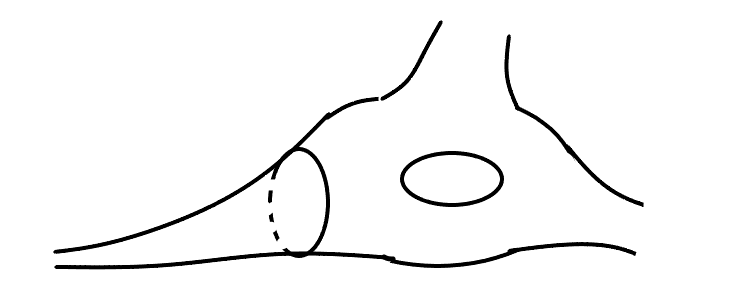
\includegraphics[width=3 in]{picture/cusp.png}
    \caption{Cusp}
    \label{fig:cusp}
\end{figure}


When the length  of some  boundary component  of the surface $S$  is zero, $S$ is a punctured  surface, and the neighborhood of the boundary component  is called a cusp. More concretely, a cusp is   the quotient domain $\{x+iy\in H|y\geq 1\}/(Tz=z+p)$ of area $p$. The horocycles $y=a$ are  corresponding to curves of length $\frac{1}{a}$ for all $a\geq 1$, they lie in the same isotopy class which contains no closed geodesic, and the minimum sequence tend to the infinity. 

For punctured surface, use $\beta_i$ to denote  the corresponding cusp instead of the boundary component, and define $F_i$, $F_{i,j}$ similarly. 




 Greg McShane prove the McShane identity in \cite{McShane1998SimpleGA} for Riemann surfaces with cusps.

\begin{theorem}[McShane identity]\label{Mcshaneid}
\begin{equation}\label{Mcshaneidorig}
    \sum_{\alpha,\beta}\frac{1}{1+\exp\left(\frac{l_\alpha(X)+l_\beta(X)}{2}\right)}=\frac{1}{2},
\end{equation}
Where the sum is taken over all the unordered  pairs $(\alpha,\beta)$ of simple closed geodesics or cusps bounding  a pair of pants with a fixed cusp. 
\end{theorem}

Mirzakhani generalizes the identity to Riemann surface with positive boundary lengths in \cite{Mirzakhani:2006fta}. 

\begin{theorem}[McShane--Mirzakhani identity]
For $X\in \mathscr{T}_{g,n}(L)$ with negative Euler characteristic,  then \begin{equation}\label{McMiid}
\sum_{\{\gamma_1,\gamma_2\}\in F_1}D(L_1,l_{\gamma_1} (X),l_{\gamma_2}(X))+\sum_{i=2}^n\sum_{\gamma\in  F_{1,i}}R(L_1,L_i,l_{\gamma}(X))=L_1.
\end{equation}
Here $L=(L_1,\cdots,L_n)$ are the length of boundary components.
\end{theorem}

Take the derivative of  the McShane--Mirzakhani identity with respect to $L_1$ at $L_1=0$ from the direction $L_1>0$. According to (\ref{pp1}) and (\ref{pp2}), the following corollary holds:

\begin{corollary}
For $X\in \mathscr{T}_{g,n}(0,L_2,\cdots,L_n)$ and $3g-3+n>0$,
\begin{equation}\label{derivMc}
    \sum_{\{\gamma_1,\gamma_2\}\in F_1}\frac{1}{1+e^{\frac{l_{\gamma_1}(X)+l_{\gamma_2}(X)}{2}}}+\sum_{j=2}^n\sum_{\gamma\in F_{1,j}}\frac{1}{2}\left(\frac{1}{1+e^{\frac{l_\gamma(X)+L_j}{2}}}+\frac{1}{1+e^{\frac{l_\gamma(X)-L_j}{2}}}\right)=\frac{1}{2}.
\end{equation}
\end{corollary}

\begin{remark}
The summation of infinity numbers and the derivation can exchange since the all terms are positive with positive derivations.
In (\ref{derivMc}), let $L_i=0$ for $i=2,3,\cdots,n$, it is the same as (\ref{McMiid}). 
\end{remark}

Note that in (\ref{McMiid}), $L_1$ is the length of boundary component $\beta_1$,  $D$ and $R$ are the length of arc on $\beta_1$ with respect to the pair of pants bounded by $\beta_1,\gamma_1,\gamma_2$ or $\beta_1,\beta_j,\gamma$. So to prove (\ref{McMiid}), separate $\beta_1$ into different pieces and calculate the length of all pieces will help. Meanwhile, it is necessity to show they are disjoint and the complement of their union is of measure zero.

A geodesic is called complete if it is not contained in another geodesic strictly. For a point $x\in \beta_i$, use $\gamma_x$ to denote the unique complete simple  geodesic passing $x$ and meeting with $\beta_i$ perpendicularly. $\gamma_x$ may the the shortest simple geodesic connecting $\beta_i$ and some $\beta_j$ in the homotopy class of finite length, it may also intersect itself at finite length and stop, otherwise it may be of infinite length and spiral around an asymptotic  geodesic.  

\begin{remark}
For a cusp domain of area $p<2$, a complete geodesic that enter it must be of the form $\{x=x_0\}$, which can be seen as orthogonal to the cusp. The original proof for McShane identity and the proof for the generalized identity are similar. 
\end{remark}


Define $E(X)$ to be the union of all simple complete geodesics which have a right intersection angle  at each meeting point with boundary components. $E_i=E(X)\cap \beta_i$ is its intersection with $\beta_i$. In figure \ref{fig:pantshy}, $y_1,y_2,z_1,z_2,w_1,w_2\in E_i$. They cut $\beta_1$ into arcs of length $\frac{1}{2}D(l_{\beta_1}(X),l_{\beta_2}(X)$, $l_{\beta_3}(X)),l_{\beta_1}(x)-R(l_{\beta_1}(X),l_{\beta_2}(X)$, $l_{\beta_3}(X)),l_{\beta_1}(x)-R(l_{\beta_1}(X),l_{\beta_3}(X),l_{\beta_2}(X))$. 
\begin{lemma}\label{measurezero}
$E_i\subset \beta_i$ is of measure zero.
\end{lemma}

\begin{proof}
Double $X$ along $\partial X$ to get $\hat{X}$. Consider the collar neighborhood $T(\beta_o)$ along $\beta_i$. Then the metric is $d\rho^2+l(\beta_i)^2\cosh^2\rho dt^2$ under the cylinder representation. For $x\in E_i$, the geodesic $\tilde{\gamma}_x$ on $\hat{X}$ passing $x$ perpendicularly is of the form $t=c$ for $c$ a constant.  For $x\neq y\in E_i$,  $\tilde{\gamma}_x\cap T(\beta_i)$ and $\tilde{\gamma}_y\cap T(\beta_i)$ are disjoint.
It follows $$\mu(\{\tilde{\gamma}_x|x\in E_i\}\cap T(\beta_i))=2 \mu(E_i)\cdot \sinh w(\beta_i)$$, where $w(\beta_i)$ is the half width of the collar $T(\beta_i)$.
By the definition of $E_i$, $\tilde{\gamma}_x$ is a  complete geodesic. By \cite{BIRMAN1985217}, the union of simple complete geodesic on $\hat{X}$ is of measure zero.
So $\mu(\{\tilde{\gamma}_x|x\in E_i\}\cap T(\beta_i))=0,$ which  implies $\mu(E_i)=0.$
\end{proof}



For $X\subset Y$, call $x\in X$ isolated if there is an open neighborhood $U$ in $Y$ of $x$ such that $U\cap X=\{x\}$. Call $x\in X$ a boundary point if $x$ is a limit point in $X$, or there exists a sequence $\{x_n\}$ of different elements in $X$ converging to $x$, and there exists a connected open set $U$ contained in $Y\backslash X$ such that $x\in \overline{U}$. Notice that this definition of boundary point is stronger than that in basic topology.


 \begin{figure}[h]
     \centering
     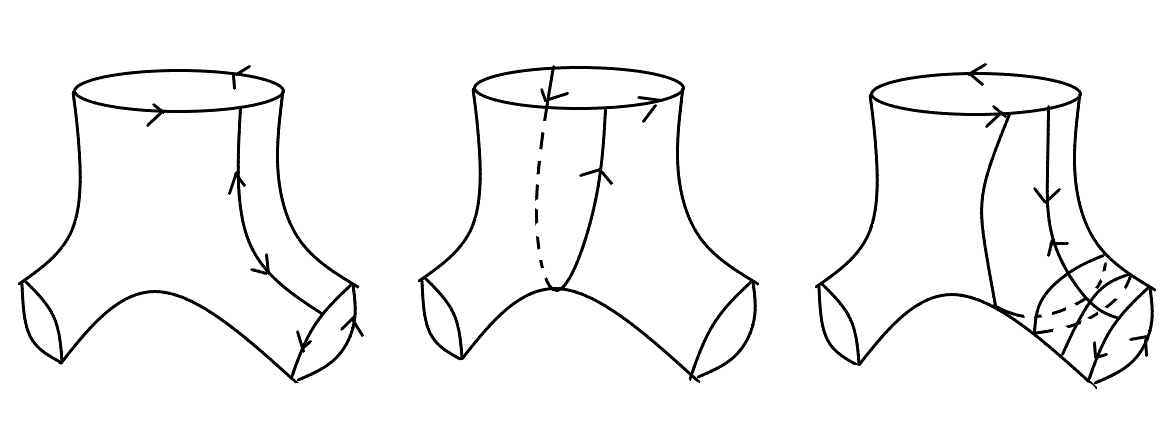
\includegraphics[width=5 in ]{picture/findpants.png}
     \caption{Pants containing $\gamma_x$}
     \label{fig:findpants}
 \end{figure}

For $x\in E_i$ connecting $\beta_i$ and $\beta_j$, there is always a canonical  method to find a pair of pants containing $\beta_i$, $\beta_j$ and $\gamma_x$.  If $\beta_i\neq \beta_j$, then consider $\beta_i\cup\gamma_x\cup\beta_j$ as a closed curve, with $\gamma_x$ twice. Among its homotopy class there is a unique simple closed geodesic $\gamma$ which bounds a pair of pants along with $\beta_i,\beta_j$. See figure \ref{fig:findpants}.  If $\beta_i=\beta_j$, then $\beta_i$ is cut into two pieces $\gamma_a,\gamma_b$, and consider the unique simple closed geodesic $\gamma_1$ in the homotopy class of $\gamma_a\cap \gamma_X$ and the unique simple closed geodesic $\gamma_2$ in the homotopy class of $\gamma_b\cap  \gamma_x$. Then $\gamma_1,\gamma_2$ bound a pair of pants along with $\beta_i$. If $\gamma_x$ spiral around $\gamma$, then is can be seen as the union of  a minimal   geodesic arc $\gamma_{x_0}$ between $\beta_i$ and $\gamma$, with an infinite  copies  of $\gamma$, find the pair of pants $P$ containing $\gamma,\beta_i$, and $\gamma_{x_0}$, then it will contain $\gamma_x$.  


According to McShane \cite{McShane1998SimpleGA}, there is a closed relationship   of topology of $x$ in   $ E_i\subset \beta_i$ and the behavior of $\gamma_x$.

\begin{theorem}\label{classify}
Points $x\in E_i$ can be classified as follows:
\begin{enumerate}
    \item If the other end of $\gamma_x$ approaches some $\beta_j$, then $x$ is isolated.
    \item If $\gamma_x$ spirals around a non-peripheral simple closed geodesic, then $x$ is a boundary point.
    \item Otherwise, $x$ is neither isolated nor a boundary point.
\end{enumerate}
\end{theorem} 

\begin{remark}


For the first case, the other end of $\gamma_x$ approach a boundary component have two possible situations. $\gamma_x$ may be the shortest geodesic connecting two boundary components and meeting them orthogonally,  or it will spiral around another boundary component and have finite length. Consider this in the pair of pants contains the geodesic and the two end boundary components.  In figure \ref{fig:pantshy}, if $\beta_1$ and $\beta_3$ are boundary components, then $y_1,y_2\in E_1$ are isolated, and the end point $x\in \beta_1$ of shortest geodesic connecting $\beta_1,\beta_3$ is isolated. For $x$, the arc $(y_1,y_2)$ which doesn't contain $w_i$, is the maximal open neighborhood the intersection of which with  $E_1$ is $\{x\}$. For $y_1$, the arc $(x,w_1)$ is the maximal open neighborhood the intersection of which with  $E_1$ is $\{y_1\}$. No matter whether $\beta_3$ is a boundary component, $w_1,w_2$ are isolated, and $(y_1,z_1)$ is the maximal open neighborhood the intersection of which with  $E_1$ is $\{w_1\}$.

For the second case, also consider it in the pair of pants contains the geodesic and the boundary component along with the asymptotic geodesic. In figure \ref{fig:pantshy}, if $\beta_3$ is non-peripheral, then $y_2,y_3\in E_1$ are boundary points, and the interval $(y_1,w_1)$ which doesn't contain $y_2$  is contained in $\beta_1\backslash E_1$. The sequence ${\gamma_{x_n}}$ contained in $E_i$, which convergent to $\gamma_{y_1}$, is   given by straightening $T^n(\gamma_x)$. Here $T\subset \Mod_{g,n}$ is the Dehn twist along $\beta_3$.  
\end{remark}




\begin{theorem}\label{Cantorset}
$E_i$ is the  union of a Cantor set and countably many isolated points.
\end{theorem}
\begin{proof}
For a subset of $[0,1]$, if it's closed with no isolated point, compact, and  totally disconnected , then 
 it is  homeomorphic to the Cantor set \cite{topologycantor} .
 
 
For isolated points in $E_i$, it is embedded into a pair of pants contained at least two boundary components, and the third boundary geodesic corresponding to  an element in the fundamental group. Since $S_{g,n}$ is a finite CW complex, by van Kampen's theorem, its fundamental group is finitely generated, so is countable.   

Notice that the Cantor set $C$ can be seen as the real number in $[0,1]$, one ternary representation $(a_0.a_1a_2\cdots)_2$ of which satisfies $a_i\neq 1$.  If $x=(a_0.a_1a_2\cdots)_2$  satisfies  only finite $a_i$ are $0$, or only finite $a_i$ are $2$, then $x\in C$ is boundary point, otherwise $x$ is not boundary point.  This corresponds to the second and third cases in theorem \ref{classify}.
\end{proof}



\begin{proof}[Proof of Theorem \ref{Mcshaneid}]
The complement of a Cantor set in $[0,1]$ is the  union of 
disjoint open intervals.

Define $I_i$  to the set of isolated points in $E_i$. By theorem \ref{Cantorset}, assume that $$
I_i\cup (\beta_i\backslash E_i)=\cup_{h}(a_h,b_h),
$$
 the union of disjoint intervals.  
 
 By definition, $a_h$ and $b_h$ are boundary points in $E_i$.
Assume that $\gamma_{a_h}$ spirals around $\Omega(\gamma_{a_h})$, which is not a boundary component.  Consider  the unique embedded pair of pants $\Sigma$ which contains $\beta_i$ and $\gamma_{a_h}$ entirely, and $$
\partial \Sigma=\{\beta_i,\Omega(\gamma_{a_h}),\gamma\}.
$$
In $S_{g,n}$, $\Omega(\gamma_{a_h})$ and $\gamma$ may overlap, but in $\Sigma$ they are cut apart and distinct. $\gamma$ may be another boundary component. 

Consider $\gamma_{b_h}$, it must spiral around $\Omega(\gamma_{a_h})$ or $\gamma$. Calculate  the length  $|b_h-a_h|$ of each interval for the two cases.

If $\Omega(\gamma_{b_h})=\Omega(\gamma_{a_h})$, then $\gamma$ must  a boundary component $\beta_j$, so $\Omega(\gamma_{a_h})\in F_{i,j}$. The interval of $(a_h,b_h)$  is of length $$ |b_h-a_h|=R(L_i,L_j,l_{\Omega(\gamma_{a_h})}(X)).$$
While if $\gamma_0\in F_{i,j}$, see $\Sigma$ in Figure \ref{fig:pantshy}. Assume  that $\beta_1$ and $\beta_2$ are boundary components of $S_{g,n}$ and $\beta_3$ is not. $\beta_3\in F_{1,2}$. Then $y_1$ and $y_2$ are boundary points in $E_1$, and they are  the limit points of a sequence in $E_1\cap (y_1y_2)$. Here $(y_1y_2)$ doesn't contain $w_i,z_i$. $E_1-[y_1,y_2]$ contains only five isolated points, $z_1,z_2,w_1,w_2$, and the meeting point of $\beta_1$ and the shortest geodesic connecting $\beta_1$ and $\beta_2$. 
 
Thus there is a one to one correspondence between intervals $(a_h,b_h)$ with $\Omega(\gamma_{a_h})=\Omega(\gamma_{b_h})=\gamma$ and $\gamma\in F_{i,j}$.


If $\Omega(\gamma_{b_h})=\gamma$, then $\gamma$ is not a boundary component and $\{\Omega(\gamma_{a_h}),\gamma\}\in F_i$. The interval $(a_h,b_h)$ is of length $$|b_h-a_h|=\frac{1}{2}D(L_i,l_{\Omega(\gamma_{a_h})}(X),l_{\gamma}(X)).$$ 
Notice that the image of $(a_h,b_h)$ under the reflection  $\sigma$ is also an open interval in $I_i\cup (\beta_i\backslash E_i)$ with the same length. So when calculate the sum of the length of all intervals, $\frac{1}{2}D(L_i,l_{\gamma_1}(X),l_{\gamma_2}(X))$ should be added twice  for $\{\gamma_1,\gamma_2\}\in F_i$.

Thus there is a two to one correspondence between intervals $(a_h,b_h)$ with $\gamma_1=\Omega(\gamma_{a_h})\neq \Omega(\gamma_{b_h})=\gamma_2$ and $\{\gamma_1,\gamma_2\}\in F_i$.
 
Since $E_i$ is of measure zero by lemma \ref{measurezero}, the $L_i=\sum_{h}|a_h-b_h|$. By the correspondence above, it is of the form 
\begin{equation*}
\sum_{\{\gamma_1,\gamma_2\}\in F_i}D(L_i,l_{\gamma_1} (X),l_{\gamma_2}(X))+\sum_{j\neq i}\sum_{\gamma\in  F_{i,j}}R(L_i,L_j,l_{\gamma}(X))=L_i.
\end{equation*}
\end{proof}


\printbibliography

\end{document}
